%%%%%%%%%%%%%%%%%%%%%%%%%%%%%%%%%%%%%%%%%%%%%%%%%%%%%%%%%%%%%%%%%%%%%%%%%%%%%%%%%%%%%%%%%%%%%%%%%%%%
\documentclass[msc]{infthesis}


%===================================================================================================
\usepackage[utf8]{inputenc}
\usepackage[T1]{fontenc}
\usepackage{fixltx2e}
\usepackage{graphicx}
\usepackage{longtable}
\usepackage{float}
\usepackage{wrapfig}
\usepackage{rotating}
\usepackage[normalem]{ulem}
\usepackage{amsmath}
\usepackage{textcomp}
\usepackage{marvosym}
\usepackage{wasysym}
\usepackage{amssymb}
\usepackage{hyperref}
\tolerance=1000
\usepackage{graphicx}
\usepackage{definitions}


%===================================================================================================
\bibliographystyle{plain}


%===================================================================================================
\newcommand{\weightedsum}[2][]{Z_{#1}^{(#2)}}
\newcommand{\weight}[2]{w_{#1}^{(#2)}}
\newcommand{\weights}[2][]{W_{#1}^{(#2)}}
\newcommand{\activation}[2][]{x_{#1}^{(#2)}}
\newcommand{\nonlinearity}[1]{g^{(#1)}}
\newcommand{\bias}[2][]{b_{#1}^{(#2)}}
\newcommand{\of}[1]{\left(\,{#1}\,\right)}
\newcommand{\norm}[1]{\left\lvert\,{#1}\right\rvert}
\newcommand{\TODO}[1]{\textbf{[TODO: {#1}]}}
\newcommand{\relu}{\operatorname{relu}}
\newcommand{\lrelu}{\operatorname{lrelu}}



\author{Daniel Wyeth}
\date{\today}
\title{Brain Tissue Segmentation via Deep Convolutional Neural Networks}


%===================================================================================================
\begin{document}

\maketitle
\tableofcontents




%%%%%%%%%%%%%%%%%%%%%%%%%%%%%%%%%%%%%%%%%%%%%%%%%%%%%%%%%%%%%%%%%%%%%%%%%%%%%%%%%%%%%%%%%%%%%%%%%%%%


\section*{foreword}

This project started out with two objectives: the first was to successfully segment several
significant neural tissue classes in MRI brain images by deep convolutional neural networks;
the second was to investigate methods by which to integrate prior information into the networks
in order to improve their performance on this task.  To the author's regret, this paper deals
only with the first of these.  In order to facilitate the implementation of the nonstandard
architectures which the second goal was expected to require, it was decided to implement the
framework for defining and training the networks from only basic components.  While this has
been an educational experience, the progress made was considerably less than would have been
the case had a standard network package been used instead.  The requirement to deal with all
of the lowest level aspects of network construction, from initialisation schemes, to adaptive
learning rates and all the other components of the optimiser pipeline has left no time for
actually making use of this infrastructure to do something which the existing fraeworks could
not, and of course in all other respects it is far more limited than they are.

My decision in the final days of work was thus to reframe the project: it would instead be
focussed on a clear and detailed analysis of the full pipeline required to build a network
which could solve the first problem.  And solve it, it does.  Despite several difficult to
track down bugs in the optimiser, in GPU memory allocation, and the last minute accidental
deletion of a large part of the experimental results, the implementation of the software
made available at:
\begin{verbatim}
    https://github.com/substructural/deep-random-fields
\end{verbatim}
achieves DICE results of \(\sim 0.8\) which, while not class leading, would still place well
in many benchmarks.  While the analysis given is obviously rushed in many places, it does I
think succeed in giving a more detailed insight into the design and function of a workable
neural network solution to a medical imaging problem than is possible in the short form of
most published papers.

To my supervisor and the friends who voiced misgivings at my hubris, let me say that your
concerns were correct, but that I hope the outcome of my mistake makes it an enlightening
one.

Daniel Wyeth


%===================================================================================================
\chapter{introduction}
\label{sec-1}


This paper documents an inestigation into the application of deep convolutional neural networks
for the segmentation of neural tissue classes in T1 weighted MRI scans of the human brain.  This
is a challenging problem, both due to the complexity of the regions to be segmented, and the
volume of data which must be processed in order to do so.  In this brief chapter we outline
the clinical motivation for this task, and then a brief overview of the problem from the
perspective of image analysis.


%===================================================================================================
\section{clinical background}
\label{sec:introduction:clinical}

The tissue classes which we aim to segment are Grey Matter (consisting of neural cell bodies),
White Matter (consisting of the axons and fibres connecting neurons), Cerebral Spinal Fluid (or
CSF, which surounds neural structures within the cranium, and background, consisting of all other
structure present in the images.  The segmentation of these tissue types is important for a number
diagnostic procedures, in particular those applied to suspected cases of neuro-degenerative
disorders such as dementia (grey matter degeneration) and multiple sclerosis (an auto-immune
disease resulting in white matter lesions).


%---------------------------------------------------------------------------------------------------




%===================================================================================================
\section{brain tissue segmentation}
\label{sec:introduction:segmentation}


The segmentation of brain structures in MRI has a very active literature,
with far too many significant papers to cover them all in depth in the introduction.  Instead
we have taken the unusual approach of integrating a discussion of the literature along with
our very extended method sections in chapters 2 and 3.  As an overview however:
\begin{itemize}
\item The dominant machine learning
  method in the first part of the decade was the Random Decision Forest,
  popularised in part by its
  use in the Microsoft Kinnect.  Pereira et al 
  \cite{Pereira:automatic-brain-tissue-segmentation-using-RDFs} is a representative
  implementation of this approach.
\item For deep learning approaches, thos most influential on our approach are:
  \begin{itemize}
  \item Brebisson and Montana
    \cite{Brebisson:deep-NN-anatomical-brain-segmentation} This paper
    investigates applying a deep convolutional neural network to the
    segmentation of cortical regions in MRI images (the MICCAI
    challenge)
  \item Kleesiek et al \cite{Kleesiek:deep-MRI-brain-extraction} The
    authors evaluate the use of a deep convolutional neural network to
    segment the whole brain (skull stripping) from multiple types of
    MRI sequences.
  \item Kamnitsas et al \cite{Kamnitsas:multi-scale-3D-CNN-with-CRF}
    This paper evaluates the application of deep convolutional neural
    networks to the segmentation of brain lesions of multiple types.
  \end{itemize}
\item This last paper is interesting in its use of both a convolutional
  neural network to provide a classification based on local image 
  information, and a conditional random field, to capture more global
  constraints.  This appoach is taken to its logical conclusion --- the
  direct inclusion of the CRF into the CNN --- in  
  Zhang et al \cite{Zhang:deep-CNNs-multi-modality-brain-segmentation}
\end{itemize}



%---------------------------------------------------------------------------------------------------
\newpage







%%%%%%%%%%%%%%%%%%%%%%%%%%%%%%%%%%%%%%%%%%%%%%%%%%%%%%%%%%%%%%%%%%%%%%%%%%%%%%%%%%%%%%%%%%%%%%%%%%%%
\chapter{classification networks}
\label{sec:classification}




%===================================================================================================
\section{basic feed forward networks}
\label{sec:classification:1}



%---------------------------------------------------------------------------------------------------


%---------------------------------------------------------------------------------------------------
\subsection{network structure}
\label{sec:classification:feed-forward:structure}


A neural network is a directed graph of functions of the form:
%
\begin{align}
%
f( x ) = g\of{ \sum_{i \in I}\of{ w_{i} x_i } + b}
%
\end{align}
%
where \(g\) is a non-linear function, normally called the activation function and \(w\) is 
is a matrix of weights.
%
In a feed forward network the graph is acyclic, and in the simplest case of a dense network, in
which every node at one layer is connected to every node at the next, can be thought of as a
simple finite sequence in which every function at a given depth in the graph has the same
activation function.
%
For such a network, each layer \(k\) can be represented by a vector valued function of the form:
%
\begin{align}
f\of{ \activation{k} }
  &=
    \left\langle
    g\of{ \sum_{i \in I}\of{ \weights[1,i]{k} \activation[i]{k} } + \bias[1]{k} },
    \ldots,
    g\of{ \sum_{i \in I}\of{ \weights[n,i]{k} \activation[i]{k} } + \bias[1]{k} }
    \right\rangle
    \\
  &= \langle g( \weights[1]{k} \cdot \activation{k} ), \ldots, g( \weights[n]{k} \cdot \activation{k} ) \langle
  \\
  &= \hat{g}( \weights{k} \activation{k} )
\end{align}
%
which applies \(g\) element wise over the dot product of each node's weight vector with 
the input vector, or equivalently, applies a vector valued variant \(G\) of \(g\) over
the matrix product of a weight matrix \(W\) (the concatenation of the individual node 
weights) and the input vector.  For brevity we will use \(\weightedsum{k}\) to denote
the vector of weighted sums:
\begin{align}
  \weightedsum{k}
  &=
  \langle\weights[1]{k}\activation{k}, \ldots, \weights[1]{k}\activation{k}\rangle
\end{align}
% 
More complex graphs are of course possible: we will meet networks which take the form of a tree,
with multiple distinct inputs to each layer, in chapter \ref{sec:segmentation}.  Networks whose
graphs admit cycles are called recurrent, and allow for the incorporation of memory into the
network; we will consider networks of this form in chapter \ref{sec:prior} when we consider
the integration of more complex probabilistic graphical models into the network.




%---------------------------------------------------------------------------------------------------
\subsection{network computation}
\label{sec:classification:feed-forward:computation}


Neural networks can be trained to compute highly non-linear functions of almost arbitrary
complexity.  Theoretical results exist which demonstrate that any continuous function can be
approximated by a neural network with one hidden layer, while a network with two hidden layers
can compute any piecewise continuous function.\cite{csaji2001approximation}

\begin{itemize}
    \item \emph{regression.}
    The process of learning a continuous real function, is called regression, and the resulting
    network a regressor.  Multiple-regression learns a mapping from the input to a vector of
    real values.  We will see an example of this in \ref{chp:prior-information} where we
    learn a mapping from an image to the parameters of an affine transformation matrix which
    registers that input to another image (actually to a probabilistic atlas).

    \item \emph{classification.}
    The complement to regression is classification: a mapping from the input domain into a 
    finite discrete set of values, which can be interpretted as a set of labels or classes for
    that data.  In practice, we would normally implement classifcation probabilistically, in
    which case the mapping is actually from the input domain to a vector of real values in 
    \([0,1]\) which form a discrete probability distribution over the classes.

    \item \emph{segmentation.}
    Most of the networks considered in this work are classifers which map input pixels to 
    a label which describes the tissue type captured at that position in the image.  Viewed
    as a partition on the image, this labelling defines a segmentation.
\end{itemize}




%===================================================================================================
\section{learning in a network}
\label{sec:classification:2}


%---------------------------------------------------------------------------------------------------
\subsection{concepts}
\label{sec:classification:concepts}
The weights in the network represent the learnable parameters of its functions.  Given a method of measuring
the difference between the output of the network for a given input, called the cost or the loss, 
and the target output for that input, we can use optimisation to iteratively update the weights so 
as to minimise this loss, and so learn the target function.


\paragraph*{gradient descent.}
The standard optimisation method used for neural networks is gradient descent: given a loss \(L\) expressable
as a differentiable function of the parameters \(w_i\) of the network, we update the network by:
%
\begin{align}
  \label{eq:gradient-descent}
w_i \longleftarrow \phi\of{ \derivative[L]{w_i} }
\end{align}
%
In the simplest case \(\phi(d) = \lambda d\) is a simple constant multiple of the derivative, in which
case \(\lambda\) is known as the \emph{learning rate}.


\paragraph*{epochs and batches.}
In order to optimise the network in this way requires a dataset of training examples consisting of input 
and output pairs.    
%
One iteration over the full dataset is called an epoch, and in the simplest case the loss \(L\)
is computed as the sum of losses over all training examples. The primary advantage of this
scheme is that the loss takes into account the performance of the network on the full variation
of inputs (to the extent that the training set represents this).
%
As learning will normally require a large number of updates to converge on an optimimal
solution, this method has the disadvantage being very slow.  Even small networks for simple
functions may require thousands of updates to converge, while a large dataset may take hours per
epoch, which together give rise to training times in the thousands of hours.  For large
networks, learning complex functions, such a method ceases to be feasible at all.

The alternative extreme is to update the parameters after each randomly selected training example, in a
process called stochastic gradient descent.
%
This has the advantage of learning very quickly, but due to the fact that the network cost is
determined by a single example at a time, it can lead to a highly erratic sequence of weight
changes.  To see this, consider a classification problem in which, for each class, there is one
parameter and one threshold which would result in perfect sensitivity to that class, but
suboptimal specificity for all other classes.  On each example, the optimal gradient results in
a change to this parameter, but to the detriment of the other classes.  While single example
learning schemes have a place in online learning applications (in which training data is
generated interactively with a user) it will be suboptimal for our use case here.

The compromise solution almost universally used in practice \cite{Glorot10understandingthe} is to divide the training
set into smaller randomly selected \emph{batches}, with the loss calculated after each batch's
completion.  In a highly vectorised implementation it would be common to use the maximum number
of examples which can be simultaneously processed as the size of the batch.  This approach,
called stochastic minibatch, is the approach which we have adopte in this work.\footnote{ Note
that the number of training examples which be simultaneous processed is dependent on the in
memory representation of those examples at each stage in the prcessing pipeline, which is itself
dependent on the structure of the network.  For this reason the batch size will necessarily
differ between different networks.}


\paragraph*{back propagation.}
The key insight which allows gradient descent to be efficiently applied to the optimisation of the network, is that 
being a composition of differentiable functions, the derivative of the loss at the \(k\)-th layer 
decomposes according to the chain rule. 
%
Specifically, the derivative of the loss with respect to each parameter, decomposes into the derivative 
of the loss with respect to the non-linear function at that layer, multiplied by the sum of the derivatives 
of the linear components with respect to that parameter.
%
\begin{align}
\derivative[ L ]{ \weights[j,i]{k} }
&=
\derivative[ L ]{ \activation{k+1}}
\cdot
\derivative[ \activation{k+1} ]{ \weights[j, i]{k} }
\\
&=
\derivative[ L ]{ \activation{k+1}}
\cdot
\derivative[ \activation{k+1} ]{ \weightedsum{k} }
\cdot
\derivative[ \weightedsum{k} ]{ \weights[j, i]{k} }
\\
&=
\derivative[ L ]{ \activation{k+1}}
\cdot
\derivative[ \nonlinearity{k}( \weightedsum{k} ) ]{ \weightedsum{k} }
\cdot
\derivative[ \weightedsum{k} ]{ \weights[j, i]{k} }
\end{align}
%
Factorising the network in this way allows us to compute the gradients for each layer using the
already computed gradients for the layer above.





%---------------------------------------------------------------------------------------------------
\subsection{saturation.}
\label{sec:classification:learning:saturation}

Learning by gradient descent depends crucially on the existence of the gradient which is to be
descended at all non-optimal points.  There are however many factors which can significantly
diminish the gradient even in the presence of significant loss relative to the target function.
We consider the most significant below.


\paragraph*{derivative of the linear sum.}
\label{sec:classification:2-2-1}
It is instructive at this point to consider the gradient of the weighted sum w.r.t. each weight
\(\weight{i,j}{k}\):
\begin{align}
  \derivative[{ \weightedsum[j]{k} }]{ \weights[j,i]{k} }
  &=
  \derivative[{ \weights[j]{k} \cdot \activation{k} }]{ \weights[j,i]{k} }
  \\
  &=
  \derivative{\weights[j,i]{k}} \of{ \sum_{i'} \weights[j,i']{k} \activation[i']{k} } 
  \\
  &=
  \derivative{ \weights[j,i]{k} } \of{  \weights[j,i]{k} \activation[i]{k} }
  \\
  &=
  \activation[i]{k}
\end{align}
%
Given that the input \(\activation[i]{k}\) is, at all layers above the first, the output of the
\(i\)-th output of the layer below, this implies that weights for layers whose inputs tend to
lie close to 0 will learn slowly, if at all.  If such activations never fire, then this is
unproblematic, but if they respond to strongly to outliers in the data, then it is worth noting
that they will do so with an effectively random unlearned weight.  This is a consideratino which
must be borne in mind when considering the shape of activation functions as well as input data
normalisation schemes.


\paragraph*{backpropagation terminates at 0 weights and 0 activation gradients.}
\label{sec:classification:2-2-1-1}
Conversely, consider the gradient of the activation:
%
\begin{align}
    \derivative[L]{ \activation[i]{k} }
    &=
      \sum_{j}\of{
      \derivative[L]{ \weightedsum[j]{k} }
      \cdot
      \derivative[{ \weightedsum[j]{k} }]{ \activation[i]{k} }
      }
    \\
    &=
      \sum_{j}\of{
      \derivative[L]{ \weightedsum[j]{k} }
      \cdot
      \derivative[{ \weights[j]{k} \activation{k} }]{ \activation[i]{k} }
      }
    \\
    &=
      \sum_{j}\of{
      \derivative[L]{ \weightedsum[j]{k} }
      \cdot
      \weights[j,i]{k}
      }
\end{align}
%
This has two immediate consequences.  The first is that no loss is propagated back through a
node if the gradient of the weights which combine with is are 0; this has implications for the
random initialisation of weights if the distribution has 0 mean.  The more problematic consequence
however is that a 0-gradient for the loss with respect to the linear sum also halts back-propagation
and this condition is much easier to trigger.  Consider that this term itself decomposes into a
product:
\begin{align}
  \derivative[L]{ \weightedsum[j]{k} }
  &=
    \derivative[ L(\activation{k+1}) ]{ \activation{k+1} }
    \cdot
    \derivative[ \activation{k+1} ]{ \weightedsum[j]{k} }
    \\
  &=
    \derivative[ L(\activation{k+1}) ]{ \activation{k+1} }
    \cdot
    \derivative[ \nonlinearity{k+1} \of{ \weightedsum[j]{k} }]{ \weightedsum[j]{k} }
\end{align}
Hence the behaviour of the non-linear loss function \(L\) and non-linear activation function
\(\nonlinearity{k+1}\) are crucial: if either of these has flat regions in their image which
do not correspond to optima in the parameter space, then the gradient carried back to the inputs
to the layer will be 0, and learning will cease for nodes below this point.





%---------------------------------------------------------------------------------------------------
\subsection{loss functions}
\label{sec:classification:2-3}
The loss function constitutes the sole signal for the adequacy of the network as an approximation
of the target function which is to be learned.  In this section we consider both a general loss and
a loss specifically designed for classification problems such as our target application.


\paragraph*{sum and mean squared difference.}
\label{sec:classification:2-3-1}
%
The traditional cost function used for neural networks, and indeed many machine learning
algorithms, is the sum of the squared differences between the predicted output and the reference
(or expected) output according to the ground truth dataset.
%
Let \(x\) be predicted output, and \(y\) be the reference value, then the sum squared difference
is defined as:
%
\begin{align}
ssd( x, y )
&=
\sum_{i} \of{ y - x }^2
\end{align}
%
This cost strongly penalises large errors relative to the number of errors, and so is unsuited to 
applications in which it might be expected that prediction will fail badly in many cases.  Medical
images with pathological data constitute an example of such a domain, and so this is one reason
to look for alternatives in this case.

One perhaps less obvious consequence of adopting such a loss function is that the significance of
a given loss value is dependent on the size of the batch over which it is calculated.  While this
is fine for applications in which a fixed batch size is possible, it is problematic in cases where
some batches may need to be smaller than others in a single epoch (to work around image sizes which
are not divisible by a required patch size for example).  Even for cases in which batch size is
fixed for a given epoch, it may still be necessary to change the batch size for different networks,
in order to account for different memory requirements and computational resources, which means the
losses for these networks now use different scales.  Given that the scale of the loss for a given
underlying error interacts with the learning rate used to determine each update, this in turn would
necessitate choosing a learning rate based on batch size.  The simple solution to this is to use not
the sum of the errors, but the mean:
\begin{align}
msd( x, y )
&=
{1 \over B} \sum_{i} \of{ y - x }^2
\end{align}
where \(B\) is the chosen batch size.  This does not automatically determine a learning rate (as we
will see below) but it at least allows it to be chosen independently of the batch.



\paragraph*{categorical cross entropy.}
\label{sec:classification:learning:cross-entropy}
%
The categorical cross entropy is a measure of the distance between two distributions, which generalises 
the more familar binary variant as follows:
%
\begin{align}
ce( p, q )
&=
\sum_i \of{ p_i \log\of{ 1 \over q_i } }
\\
&=
-\sum_i \of{ p_i \log\of{ q_i } }
\end{align}
%
It should be noted however that the reference distribution is derived from the ground truth labelling 
of the dataset, and hence is a trivial distribution which assigns all probability mass to a single value
(i.e. to the true label for the example).  It follows that in practice the categorical cross entropy 
reduces to the uncertainty of the true label under the predicted distribution, i.e. if the true label is 
\(k\) then:
%
\begin{align}
ce( p, q ) 
&= -( p_k \log( q_k ) \\ 
&= -\log( q_k )
\end{align}
%
This then gives the loss for a single training example.  To aggregate the losses over a batch, we then
take the mean loss:
\begin{align}
mce( p, q ) 
  &=
    {-1 \over B} \sum_i \of{ p_i \log\of{ q_i } }
\end{align}
for the reasons outlined above.  This is the cost function used for the majority of the experiments
detailed in chapter \ref{sec:experiments} and if not otherwise specified, is the loss used for any
results referenced in this paper.


\paragraph*{domain specificity.}
\label{sec:classification:2-3-3-1}
Neither of these cost functions is specific to our primary task: the segmentation of medical images,
and both are in a sense more proxies for the actual error of the network, than true measures of it.
For this reason we will explore this topic further in the context of our intended application in 
chapter \ref{sec:segmentation}.





%---------------------------------------------------------------------------------------------------
\subsection{regularisation}
\label{sec:classification:2-4}


While the most obvious concept of loss derives from the error in the output of the network relative
to the target function, it is important to bear in mind that the target function itself is unknown,
and not all approximations which satisfy the sample points in the training set are equally likely to
correctly characterise it.  This observation leads to the idea of introducing terms into the loss
which penalise a parameterisation of the network, not for error on the training samples, but for the
plausibility of the structure of the network itself.  Such modification of the loss is called
regularisation, and in this section we consider its motivations, two specific regularisation terms
and some empirical results (detailed fully in chapter \ref{sec:experiments}) on their effectiveness.


\paragraph*{the preference for simplicity of explanation.}
\label{sec:classification:2-4-1-1}
Given two explanations of a body of data with equivalent accuracy but differing complexity, we would
prefer our network to choose the simpler option.  In terms of a neural network, or other machine learning
model, this amounts to a preference for models with smaller weights and a smaller number of weights
which are non-zero.  The justification for this principle is partly philosophical and partly pragmatic.

\paragraph*{the philosophical argument.}
\label{sec:classification:2-4-1-2}
Each non-zero parameter represents an empirical hypothesis that the functional relationship between
the input and output is constrained according to the effect of that parameter on the function which
it parameterises.  The more constraints are embedded in the model, the smaller the class of datasets
which satisfy them.  While the current value of the parameter is a product of optimisation on training
data, and so empirically determined in some sense, it is also a consequence of both its own random
intialisation, and the random initialisation of the other parameters.  Moreover, while it represents
a best approximation of the optimal value, given the state of the other parameters, based on that
subset of the dataset seen at this point, this sample may not be representative of the general case.
For both of these reasons its optimality consitutes an unverified assumption made on the basis of
incomplete evidence.  The fewer such assumptions a model relies on, the lower the probability that 
further evidence will undermine it, and hence the more likely it is that it will generalise.

\paragraph*{the pragmatic position.}
\label{sec:classification:2-4-1-3} Of course the primary reason that model simplification is
widely applied is that in many applications it works quite well: given two models which generate
equivalently accurate predictions on a given subset of the data, the simpler more frequently 
generalises to subsequent data than the more complex one.\cite{bishop:2006:PRML}  Of course in practice
the effectiveness of the terms is a function of both the sampling of the data, and the form of the
model, and so should be experimentally evaluated.  We present some results on this at the end of the
section.


\paragraph*{penalising the sum of non-zero parameters.}
\label{sec:classification:2-4-2-1}
The first form of regularisation which we consider uses the \(L_1\) norm is simply the 
absolute value of the parameters:
%
\begin{align}
L_1\of{\weights{k}} 
&=
\sum_{j,i} \norm{ \weights[j,i]{k} }
\end{align}
%
This term penalises the absolute sum of the weights, but is invariant to the distribution of the
weight between those parameters.  In practice applying such a cost this will drive all parameters
down at an equal rate, and hence will primarily serve to reduce small weights to 0.



\paragraph*{penalising large weights.}
\label{sec:classification:2-4-3-1}
Another measure of the complexity of a model is the number of large weights.  We can introduce a
term to penalise larger weights disproportionately over smaller ones using the \(L_2\) norm, i.e.
the square of the weight value:
%
\begin{align}
L_2 \of{ \weights{k} }
&=
\sum_{j,i} \of{ \weights[j,i]{k} }^2
\end{align}
%
The intention of this term is to decrease the absolute magnitude of the largest weights, by penalising
them more than the \(L_1\) loss would do.  While this is the case for weights greater than \(1\),
for \(\weights[j,i]{k} \in (0, 1)\) the penalty is less than that of the \(L_1\) loss given that
\(0 < x < 1\) implies that \(x^2 < x\).  This is significant for our present work in that our weights
are initialised lie well within this range.


\paragraph*{results.}
\TODO{include the \(L_1\) and \(L_2\) experiment results}




%---------------------------------------------------------------------------------------------------
\subsection{adaptive learning rates}
\label{sec:classification:2-5}


Consideration of the learning rate parameter \(\lambda\) in equation \ref{eq:gradient-descent}
will reveal two possible modes of failure, if the value is incorrectly chosen for the dataset.

The first mode occurs where the learning rate is too high, and the resulting updates to the
network cause it to oscilate, and ultimately fail to converge.  This is particularly problematic
where the gradients form a valley with steep sides roughly parallel to each other, and the
nearest local minimum lies along the valley floor in a direction almost orthogonal to the
direction of the steepest gradient at any point along the sides of the valley.  In this case
simple gradient descent will lead to updates which change sign on each batch, and if the
learning rate is too high, overstep the sides of the valley altogether, leading to divergence.
%
The lower the gradients, the less likely it is that a large learning rate will cause learning to
diverge, however this is difficult to ensure in practice.  The loss gradients which normally
arise for at least the first few iterations in training, where the weights are still largely in
the randomly initialised state, will generally be large, given that a random parameterisation is
unlikely to correctly capture the target function.  Indeed, anecdotally, it is normally during
this initial phase that learning diverges in a sequence of ever increasing losses.

An obvious
solution is to simply choose a lower learning rate, but this comes with its own problems:
if the learning rate is too small then convergence may take longer than is feasible or become
trapped in a local minimum.  The error surface of a model with as many parameters as a typical
neural network is highly non-convex, with very large numbers of local minima, and an even larger
number of shallow valleys.
%
\TODO{include experiment results to demonstrate divergence and convergence on a local minimum}
%
While it is possible to manually tune a learning rate to different phases of the optimisation,
and indeed it has been suguested that this leads to better results, \cite{goodfellow2016deep},
this is a time consuming option, and impractical during hyper parameter exploration, where large
numbers of networks must be trained and evaluated.  For this reason a number of algorithms have
been proposed to automatically adjust the effective learning rate during training.  The simplest
of these essentially serves only to escape oscilations which might lead to divergence, while the
most sophisticated reduce the learning rate when gradients are steep (and hence learning is likely to
be too fast), and an increase it where the gradient is flat (and learning is likely to be
too slow).


\paragraph*{momentum}
The core idea is to maintain a runninng estimate of the direction of optimal change, a vector
\(v\) in the same space as the parameters, which decays over time according to a hyper-parameter
\(\gamma\) and acrues changes according to the current gradient by the learning rate:
\begin{align}
  \label{eq:momentum}
  v_{0}
  &=
    0_{\weights{k}}
    \\
  v_{t+1}
  &=
    \gamma v_{t} + \lambda \nabla_{\weights{k}} L
\end{align}
The weight update is then just:
\begin{align}
  \weights{k}
  &\longleftarrow
    \weights{k} - v
\end{align}
with the new velocity term replacing the raw gradients.  The reason that this is effective in
damping oscilations is that opposing gradients (from conseuctive batches) will cancel out (to
the extent that they are of equivalent magnitude) leaving only the common components.  In our
example of a narrow valley, with nearly parallel sides and a shallow orthogonal gradient in
between them, the dominent gradients pointing across the valley will cancel, leaving only the
component orthogonal to both, pointing towards the local optimum.  Should the gradients be
large enough to skip over the opposing side of the valley in a single update of course, this
scheme will do nothing to prevent it, as it takes no account of the steepness of the gradient,
only the cancellative effect of opposing ones.


\paragraph*{adagrad}
%
This method also uses a momentum-like term which accumulates gradients but which instead uses it
as a weighting term on the learning rate.  The accumulated term (denote \(a\) below) is in
essense the sum of the squared gradients:
\begin{align}
  \label{eq:adagrad}
  a_{0}
  &=
    0_{\weights{k}}
  \\
  a_{t+1}
  &=
    a_{t} + \of{ \nabla_{\weights{k}} L }^2
\end{align}
The weight updates then proceed with a learning rate derived from \(a\) as follows:
\begin{align}
  \weights{k}
  &\longleftarrow
    \weights{k}
    -
    { \lambda \over \delta + \sqrt{a} } \nabla_{\weights{k}} L
\end{align}
%
The \(\delta\) term is a small constant intended to prevent division by 0, or indeed
the overflow which would result in the case of very small values of \(a\).
%
One obvious
limitation of this cheme is that the accumulated term grows without bound, and hence the effective
learning rate will tend towards \(0\) over time.  The next method presents one solution to this.
\cite{goodfellow2016deep}


\paragraph*{RMS prop}
%
The final adaptive method we considered, and the one which we chose to implement for our
framework, extends AdaGrad with a decay term, which prevents the accumulated gradients from
growing unboundedly, and hence does not drive the effective learning rate to 0 over time.  For
this purpose we add an additional hyper-parameter \(\rho \in (0, 1)\), called the decay term
and applied as follows:
\begin{align}
  \label{eq:adagrad}
  a_{0}
  &=
    0_{\weights{k}}
  \\
  a_{t+1}
  &=
    \rho a_{t} + (1 - \rho)\of{ \nabla_{\weights{k}} L }^2
\end{align}
The parameter update then follows the same form as for AdaGrad:
%
\begin{align}
  \weights{k}
  &\longleftarrow
    \weights{k}
    -
    { \lambda \over \delta + \sqrt{a} } \nabla_{\weights{k}} L
\end{align}
%
In our implementation we take \(\delta = 10^{-6}\) which is small enough to have little effect
when gradients are large, but large enough to prevent overflow of the effective learning rate.
\cite{goodfellow2016deep}




%===================================================================================================
\section{components of the network}
\label{sec:classification:3}



%---------------------------------------------------------------------------------------------------
\subsection{the linear weights}
\label{sec:classification:2-6}

The weights in the linear component of the network represent the learned model of the domain.  As
these are freely modified during training by the optimiser, and not managed directly, it is
imperative that they be initialised so as to allow learning to take place.  In much the same
way as using unnormalised data can lead to unmanageably large gradients for the weights,
using unnormalised weights can lead to untenably large gradients for the activations.  In both
cases learning in the network is likely to diverge with ever increasing costs which eventually
overflow.  For our implementation we have elected to initialise all weights by a 0-mean normal
distribution whose variance is determined by the combined number of inputs \(m\) and outputs \(n\)
to each node:
\begin{align}
  \label{eq:weight-initialisation}
  \weights[j,i]{k}
  &=
    N\of{ 0, { \sqrt{2 \over  m_{j,i}^{(k)} + n_{j,i}^{(k)}} } }
\end{align}
While we experimented with the use of a uniform distribution (whose range was equal to the
variance of the network above) with the expectation that this would
provide a better exploration of the parameter space, our results were highly disappointing, with
most networks initialised in this way diverging quickly, and at best converging on truly terrible
local optima.  We also experimented with different normalising constants in the numerator of the
variance term, and with the use of orthogonal weight vectors (found via singular value decomposition)
but in each case, to no good effect; sadly these experiments were abandoned prior to completion,
due to a lack of time.  See \cite{DBLP:journals/corr/SaxeMG13} and \cite{Glorot10understandingthe}
for details.


%---------------------------------------------------------------------------------------------------
\subsection{the non-linear activation function}
\label{sec:classification:3-1}


The activation function is the mechanism which introduces non-linearity to the network output,
and hence, in the case of a classifier, to the decision boundary which it determines.


\paragraph*{sigmoid}
%
The classic activation function used in the literature is the sigmoid, which maps \(\Reals\) into
the open interval \((0,1)\) as follows:
%
\begin{align}
  \label{eq:sigmoid}
  \sigma( x )
  &=
  { 1 \over 1 + e^{-x} }
\end{align}
%
The appeal of this as an function for units which map linear weighted inputs to probabilities is
obvious, and indeed its use predates multiple layer networks, deriving from ealier logistic
regressors.
%
Despite its appeal, and long history in neural networks, the sigmoid has two significant
problems as an activation function.
%
The first is that the gradients of the function tend to 0
as \(\norm{x} \approaches \pm\infty\) and so too does learning when the activation becomes very
large (either positive or negative).
%
The second is that its value lies close to 0 for inputs
negative inputs, and as we have seen, activations of 0 block the backpropagation of loss through
the network.
%
These issues have lead to a search for alternatives which do not saturated at 0 and with better
behaviour for extreme values.


\paragraph*{tanh.}
%
The hyperbolic tangent is defined as follows:
%
\begin{align}
  \label{eq:tanh}
  \tanh(x) &= { {e^{x} - e^{-x}} \over { e^{x} + e^{-x}} }
\end{align}
%
This has a very similar shape to the standard sigmoid (it is very roughly approximated by \(2
\sigma(x) - 1\)) but with a different range: \((-1, +1)\).  This change allows it to avoid the
saturation which occurs for activations near 0. Unfortunately, given its similarity in shape it
still retains the deficiency (as an activation function) that its derivative
\(\derivative[\tanh(x)]{x} \approaches 0\) as \(x \approaches \pm\infty\), and hence learning
becomes very slow as its weighted sum increases or decreases away from 0.



\paragraph*{rectified linear units}
%
The activation which has occasionally been claimed to have enabled deep learning, called ReLU
for short, is a very simple non-linearity: it takes the value of its input, for inputs greater
than 0, and 0 otherwise:
%
\begin{align}
  \label{eq:relu}
  \relu( x ) &=
    \begin{cases}
      x & x > 0 \\
      0 & \text{otherwise}
    \end{cases}
\end{align}
%
There are several features of this function, qua activation function, which deserve comment.  The
first and perhaps most obvious, is that the function is not strictly differentiable, as it is not
everywhere continuous.  It is however left and right continuous at 0, which, it turns out, is
sufficient for its use in backpropagation.
%
The second feature is its surprising effectiveness.  To see why this might be the case, consider
that:
\begin{align}
\label{eq:relu-derivative}
\derivative[\relu(x)]{x} &= 
    \begin{cases}
      1 & x > 0 \\
      0 & \text{otherwise}
    \end{cases}
\end{align}
%
It follows that relu is a perfect propagator of gradients, provided that its input is positive.
This helps to offset the vanishing gradient problem which we will discuss in
\ref{sec:classification:depth}, as it does not saturate for large (positive) values and does not
decrease the signal fed back to its linear weights.  The qualification: provided that its input
is positive turns out to be a significant one however, as \(\relu\) does most certainly saturate
for negative values, which leads us to the next variant.


\paragraph*{leaky rectified linear units}
%
The obvious modification to \(\relu\) which would work around this saturation for non-positive
values is to allow negative values to also propagate, but in a different proportion to positive
values:
\begin{align}
  \label{eq:lrelu}
  \lrelu_{\rho}(x)
  &=
    \begin{cases}
      x & x > 0 \\
      \rho x & \text{otherwise}
    \end{cases}
\end{align}
%
where the hyper-parameter \(\rho\) is often called the leakiness of the activation.  This is of
course a simple generalisation of standard \(\relu\) given that \(\lrelu_0\) is completely equivalent,
but the preservation of negative signal serves to resolve the saturation issues which standard
\(\relu\) exhibits.  For this reason this is the activation function chosen for our learned layers
in the networks used in this work.  We provide experimental justification for this coice below.


\paragraph*{results.}
\TODO{include leakiness results}



%---------------------------------------------------------------------------------------------------
\subsection{softmax and probability densities per voxel}
\label{sec:classification:3-2}

For a classification network, it is important that the final output be interpretable as a
probability distribution over the class values for the problem.  While a sigmoid activation
function ensures this for a simple binary problem, our application here is multiclass, and
of course, our activation function is leaky ReLU.  For this reason we introduce a standard
layer whose purpose is to perform this transformation.


\paragraph*{coercion to a distribution}
\label{sec:classification:3-2-1}
In order to enforce the constraint that the regressed values form a distribution, we must
apply a normalisation function.  The standard choice for this is softmax:
%
\begin{align}
p( x_i ) = { e^{x_i} \over \sum_{j} e^{x_j} }
\end{align}
%

\paragraph*{numerical issues.}
\label{sec:classification:3-2-2}
One complexity with the use of this function in practice however, is that it overflows
the representable values of most floating point types, leading to \(NaN\) values which
then cause computation to fail.  We can work around this using a technique often referred
to as the log sum exp trick.  Noting that:
%
\begin{align}
\log( c^{x} ) 
&= \log( c^{x - m + m } ) \\
&= \log( c^{x - m } c^{m} ) \\
&= \log( c^{x - m } ) + \log( c^{m} ) 
\end{align}
%
we can choose \(m = \max( x_i )\) and then reason as follows:
\begin{align}
  \label{eq:softmax-log-sum-exp}
  \log\of{ e^{x_i} \over \sum_{j} e^{x_j} }
  &=
  \log\of{e^{x_i}} - \log\of{\sum_{j} e^{x_j} }
  \\
  &=
  x_i - \log\of{\sum_{j} e^{x_j} }
  \\
  &=
  x_i - \log\of{\sum_{j} e^{x_j - m + m} }
  \\
  &=
  x_i - \log\of{e^m} - \log\of{\sum_{j} e^{x_j - m} }
  \\
  &=
  x_i - m - \log\of{\sum_{j} e^{x_j - m} }
\end{align}
%
The calculation of \(p(x_i) = {e^{x_i} \over \sum_j e^{x_j}}\) can then be done in log space using
the final expression derived above, in which only the smallest terms \(x_j\) can underflow, thus
maximally preserving the accuracy of the probability estimate.



%---------------------------------------------------------------------------------------------------
\subsection{data normalisation}
\label{sec:classification:3-4}

As discussed in section \ref{sec:classification:learning:saturation} there is a direct relation
between the magnitude of the data and the magnitude of the gradients of the network, and this
as we showed must be carefully calibrated with the magnitude of the parameters to ensure that 
the network converges on an optimal solution (or indeed converges at all).  In this section we
consider approaches to constraining the data to satisfy these requirement. 



\paragraph*{the significance of a signal.}
%
To take a philosophical perspective for a moment, the significance of a datum lies not in its value
but only in the relation betweeen that value and the other values received on a channel.  It is this
variation which needs to correspond to the variation in the underlying system in order for it to
describe that system.  This in nmind, the native units of the data are a poor choice  for the input
to the network.  A much better choice of unit is the standard deviation of the data, as this
both captures the essential signal (the degree of variation in the generating system) and also
maps it into a single scale against which the other units in the network can be calibrated.
%
More formally:
%
\begin{align}
  \label{eq:data-normalisation}
  \mu &= \expect{\activation{0}} \\
  \sigma &= \expect{{ (\activation{0} - \mu)^2 }} \\
  \hat{x} &= { \activation{0} - \mu \over \sigma }
\end{align}
This yields input data with 0 mean and unit variance, hence making standard deviation equal to 1 and
the unit just the number of standard deviations from the mean.


\paragraph*{relation between data and weights.}
%
The native units for our intended application are MRI pixel values, which are a function of a
quantum physical phenomenon, for T1, it is the time to relaxation for the quantum spin on
certain protons within the magnetic field.  While the time to relaxation is a physically
meaningful quantity, the recorded pixel values do not necessarily encode it directly, but rather
use manufacturer specific encodings.  This alone makes normalisation of the data desirable.  Even
if the values were consistent between manufacturers and scan sequences however, the sheer scale
of the values would constitute a reasno for normalising them: these values span the full \((-2^{15},
2^{15})\)
range supported by the 16 bit encoding in the data.  Even small gradients on this scale
would overwhelm our unit normal initialised weights, and lead to rapid divergence of the network.
Indeed, in our experiments, unnormalised data generally lead to NaN values in the cost function
within the first \(10\) -- \(20\) batches, depending on the batch size.


\paragraph*{validity of padding}
%
The final argument for the normalisation of the data to 0-mean is the necessity of padding.
There are several places in the pipeline where an operation may require more input values than
are actually present in the data.  In these cases we are left with a choice: we can either
restrain the application of the operation, so as to remain withing the valid input, or we can
pad the data with a synthetic value to fill out the rquired input.  The former is in some cases
(which we will consider in detail in the next chapter) far too restrictive, and so there is a
strong argument for the latter.  The problem with synthetic values however is the possibility of
creating a sythetic signal.  Ideally such padding values should have as small an effect on the
operations in which they participate as possible, and in most cases this implies that they
should deally be indistiinguishable from the surrounding data.  Using data with a 0 mean and
small variance greatly facilitates this, as the chosen mean has no effect on additive
operations, and the small variance means that most data will lie very close to the synthetic
value.


%---------------------------------------------------------------------------------------------------




%===================================================================================================
\section{representational capacity and network depth}
\label{sec:classification:depth}

The overwhelming trend in the neural network literature is torwards deeper
networks.\cite{simonyan2014very} The advantages of depth involve the increased abstraction of
features, and in the case of the convolutional architectures which we will meet in the next
chapter, an increase in the contenxtual information used in classification.  The power of such
networks is well attested, but so too is the difficulty of training training them at all: with
each layer the signal carried by the loss function attenuates and the resulting updates become
weaker.  We consider methods for working around this in section
\ref{sec:classification:deep:gradients}.  Due to their sheer size, such models can also exhibit
the opposite problem however: the large number of model parameters relative to the training
data, can allow the network to model noise in the training set, leading to overfitting and a
failure to generalise.  We consider methods for dealing with this in section
\ref{sec:classification:overfitting}.


%---------------------------------------------------------------------------------------------------
\subsection{abstraction and the feature hierarchy}
\label{sec:classification:deep:abstraction}

The power of neural networks over other machine learning algorithms is at least in part that they
learn not only the relationships between features, but the features themselves.
%
Each node in a neural network, with its linear weights and its bias serving as a threshold acts as
a simple feature detector for its input.  Where this input comes from the domain, it will most
likely capture a relatively obvious feature of the objects to be classified, the sort of feature
which one might trarditionally have coded directly if working with a machine learning algorithm
in which feature representations were not learned.  Where the input is actually the output of a
lower layer however, this is a feature of a feature.  This ever increasing abstraction in the
features learned by neural networks allows them to capture inordinately complex relationships
which are not expressable in terms of the first order attributes of the objects in the domain.
%
While the most striking examples of this sort of hierarchical feature learning (see \TODO{cite
the visualising CNNs paper} come from the convolutional neural networks (CNNs) which we will
meet in the next chapter, they are present in all networks with more than a single hidden
(non-input, non-output) layer.  Indeed, the easily visualisable features learned by CNNs are in
part easily visualisable because they are far more constrained than the features representable
by a general network.

While the techniques to be considered below allow one to train such networks, it should be observed
that high levels of abstraction do not always lead more effective classification.  The issue here
is of matching the abstraction of the feature representation to the abstraction of the problem.
To recognise human emotion in an image would seem to require a complex model of the possible
deformations of the human face, and the mapping of these to emotional states.  These are far from
first order properties of the image, and benefit enormously from increasing abstraction.  The
boundaries of tissue classes in MRI data, our target application, is not so clearly abstract
however.  Certainly shape and distribution are relevant, as is some notion of anatomical structure,
but the mapping in this case would appear to be lower level, and the absence of improvement in
our results from deeper models to some extent bears this out, though such a negative result could
equally as well arise from a deficiency in our training methods, so this is far from conclusive.


%---------------------------------------------------------------------------------------------------
\subsection{vanishing gradients}
\label{sec:classification:deep:gradients}

Begin by observing that each step in the back propagation of loss first multiplies the loss at
that layer by the gradient of the activation function (w.r.t. the linear component), and then
by the linear weight on the input.  Both of these steps will serve to reduce the gradient, the
non-linear activation function particularly so.  While the use of ReLU ad LReLU actions preserves
more of the signal, in both cases the gradient is reduced for negative weighted inputs, so in
neither case is the attenuation eliminated.  Over the course of many layers, this process may
be enough to reduce the gradient reaching a weight to almost zero, thus impeding learning.  The
more layers in the network, the more pronounced this effect becomes.  In this section we will
consider several proposed methods by which to work around this. 


\paragraph*{network pretraining}
%
Perhaps the simplest solution is to train the network in stages: one layer at a time.  For a
classification network, the classic approach would be to begin with a single hidden layer and
one classification layer, train this until convergence; the next step is to replace the existing
classification layer with two new layers: a new hidden layer and a new classification layer. At
each stage the network grows by only two layers, both of which occur at the shallowest position
in the network, and thus are least affected by the attenuation of gradients.

There are of course practical considerations in the implementation of even so simple an idea as
this.  The first is that unless a facility is added to allow trained an untrained nodes to be
intermingled, layers must be added as a whole unit, which in turn implies that the input
dimensionality of the new hidden layer must match the output dimensionality of the last
pretrained layer.

The second consideration is the status of the pretrained weights.  Consider that while the
weights in the pretrained component have been optimised to compute some set of features which
were effective in classification (with the initial classification layer), the weights in the new
layers will by default be random, and hence initially generate a large loss.  If the optimiser
is allowed to propagate the gradient of this loss back to the pretrained layers, then these will
begin to lose coherence in their computed features.  Dependant on the amount of time required
for the new layers to settle on their own useful features, the lower layers may well have
effectively unlearned much of what they could previously compute, thus obviating the benefits of
having pretrained the network.  One solution to this is to freeze the weights of the pretrained
layers, thus preserving them through the intial contortions of the new layers during the first
epoch.  This itself has consequences however: the features which were most efficacious in the
classification in the smaller network may not be the most optimal for the new larger net.  It
may be that the optimal solution is to freeze for only a limited period, and then unfreeze to
allow the new network to settle into its new structure.  Our custom network framework allows
transfer of pretrained layers with frozen weights, and also continuation of training with a
different specification of which weights are mutable, but due to limitations of time, we have
not implements support for automatically transitioning from one training regime to another.  In
consequence, a mixed training regime, in which weights change from constant to mutable, requires
a manual restart of training, which has limited our ability to explore this option fully.



\paragraph*{skip layers and residual networks}

A more recent method to improve training in deeper networks is to, perhaps somewhat
paradoxically, allow layers to ignore their inputs.  In more detail, a skip connection is an
input to a node at leyer \(k + 1\) is an edge in the graph which connects to a node, not at
layer \(k\), but rather at \(k-1\), essentially allowing the node to skip the preceding layer,
if incorporating its output does not lead to an improvement in the gradient of the loss at that
node.  The skip connection is in all other respects a normal input, and its weight in the
activation of that node is learned in the normal way.
%
\cite{he2016identity}
%
This has two effects.  First, by
effectively eliminating nodes along a path which are not strongly contributing to the accuracy
of the network, it minimises the unnecessary attenation of the gradient along that path during
back propagation.  It also seems to us however that this would serve a second purpose: it allows
features at multiple levels of abstraction to serve as inputs to a single higher level feature.
This is an increase in representational power, made possible by reducing the number of active
nodes in the network.  While skip connections are thus an appealing architectural advance, they
also require a much more flexible representation for the network, one which is capable of
representing non-sequential graph structures.  This is a feature which we have not yet
implemented in our framework, and for this reason we have not made use of skip connections
in this work.



\paragraph*{deep supervision}
%
Where skip connections attempt to preserve more of the gradient of the loss during back
propagation, the idea behind deep supervision is to provide more positions at which a
loss can be computed and back propagated from.  This idea appears in many forms (\TODO{cite
  at least a few of these} but have in common that the network has multiple output nodes at
which a loss is computed (not necessarily using the same loss function) and from which it is
then fed back.  Machanisms for aggregating loss gradients at nodes which lie on a path from
multiple supervisors include taking the mean, the median or the maximum loss.
%
\cite{lee2015deeply}



%---------------------------------------------------------------------------------------------------

%---------------------------------------------------------------------------------------------------
\subsection{overfitting and network size}
\label{sec:classification:deep:overfitting}


A network has overfit to its training set just if it models features of that data which are not
present in the general domain to which the classifier is intended to apply.  Such features constitute
noise rather than true signal, as they are not relevant to classification accurcy on the target
set.  There are many reasons why overfitting might occur, but the one of most relevance to very deep
networks concerns the relationship between the representational capacity of the network and the
size of the dataset on which it is trained.  If a classifer (or a indeed a regressor) has a complex
enough model to simply record the correct class (or real value) associated with each training example,
then this will in practice be a dominant strategy over learning a more fundmental relationship (which
may, due to noise in the data, fit the training set less well than the per example approach).

The best defence against overfitting is of course always to have a larger training set which 
perfectly represents the true domain, but in practice that is not normally an option.  Absent this,
choosing a model structure whose complexity (in terms of free parameters) is significantly less
than the number of examples on which to train it will ensure that at least some compression of the
patterns in the training set is required.  For problems with small amounts of available data however,
such as many problems in medical image analysis, this may require untenably small models.  There are
however more proactive techniques which can be used to combat the problem, which note two here.

The first strategy is to sythetically augment the training set by generating new training
examples using transformations which are known to preserve the class label.  For image based
tasks, the canonical examples are translations, mildly anisotropic scalings and small rotations
(of less than \(\pi / 4\)) which do not change the interpretation of the image.  For some
problems more general affine transformations are class preserving, allowing for arbitrary
scalings, rotations and shears.  Given a mathematical model of the natural variations of the
target shape it may be acceptable to apply non-linear transforms such as spline based
deformations, but care must be taken, particular in the context of complex anatomical structures
to preserve the natural constraints on structure which it is to be hoped the network will learn.

The second approach is to randomly perturb the activations of the network during the forward pass
in order to force the network to ignore noise.  In the extreme case, called dropout, whole nodes,
even whole subtrees of the network, are randomly ommitted from the forward pass.  The effect is to
make the network much more robust.\cite{srivastava2014dropout}

We note that for our own implementation we had not yet needed to implement any of the following, as
the number of training examples (unique 3D patches in the input) totalled approximately 
\(892 \times 10^{6}\), which is more than four orders of magnitude greater than the number of
trainable parameters in our deepest model.  Our intent had been to implement dropout however as
it 



%---------------------------------------------------------------------------------------------------




%%%%%%%%%%%%%%%%%%%%%%%%%%%%%%%%%%%%%%%%%%%%%%%%%%%%%%%%%%%%%%%%%%%%%%%%%%%%%%%%%%%%%%%%%%%%%%%%%%%%
\chapter{segmentation as classification}





\label{sec:segmentation}
In this chapter we set out those parts of our method which are specific to image processing and
segmentation.  Our focus here is much narrower than in the previouus chapter, and driven more by
empirical anlysis of our dataset than by fundmental mathematical properties of networks.  We
begin by introducing convolutional layers as position invariant features in section
\S\ref{sec:segmentation:convolution}; these will form the basis of our networks for segmentation.
In \S\ref{sec:segmentation:sliding-window} we consider how to use classification networks to generate
a segmentation, and examine some of the computational issues which arise from the na\"ive approach.
This leads naturally to a discussion of dense inference, a computationally efficient mechanism for
performing simultaneous classification or segmentation on regions of an image, detailed in
\S\ref{sec:segmentation:dense-inference}.  This approach imposes some constraints on the structure
of the network however, in that it requires the operations to be resolution preserving; we consider
the inter-relations between resolution, receptive field size and contextual information in section
\S\ref{sec:segmentation:resolutions}.



%===================================================================================================
\section{convolutional neural networks}
\label{sec:segmentation:convolution}


The simplest approach to characterising a complex object is to break it into simpler parts,
recursively if required, until we obtain components which can be directly detected.   Complex
shapes reduce to arrangements of simpler shapes, which reduce to surfaces, or curves or corners,
which themselves reduce to edges and gradients.  The hierarchical features of a neural network
provide a structure capable of representing such an a layered arrangement of increasingly
abstract features; the difficulty is in coercing the network to represent the problem in this
way.  The parameter space of even a relatively simple network is capable of modelling the data
presented to it in a bewildering variety of forms, most of which would be unintelligible to a
human observer, so the question here is most emphatically not how exapand the network's
representational capacity, but rather how to constrain it, so as to learn the sort of compositional
image features in terms of which we ourselves tend to conceptualise the problem.  Changing our
network representation from a dense graph of fully connected layers, to a sparse graph of more
plausibly connected ones is the first step in the transition.  Reframing the linear operation
as a convolution of the input with a discrete kernel is the next.  The transition to a fully
convolutional network is completed by structuring the whole network in these terms: as a network
of learnable filters transforming images at one layer of abstraction into new images giving the
feature response at each point in the input.

%---------------------------------------------------------------------------------------------------
\paragraph*{position invariance.}
%
The lowest level features which make up our target objects are largely position invariant:
the presence of an edge at a particular angle in an image is characterisable by the same linear
combination of weights applied to a region centred on it irrespective of where that region lies
in the image.
%
Unfortunately however, our dense networks are not easily able to take advantage of this fact.
Each weight attaches to the edge connecting a node with a particular input, which at the first
layer corresponds to a particular pixel, hence the linear combination of weights which detect
an edge must be learned seprately for every position in the input of the network.  Learning the
detection of edges thus requires significantly more examples than it would if the nodes which
were to learn the representation of an edge, were able to respond to any patch in the image.
%
Conceptually then what we would like is to allow the network to learn weights which are applied
not just to a single input, but together applied as a filter over a sliding window of the input.
This way of reframing the problem takes advantage of the fact that the inputs are spatially
related in a meaningful way, and uses this fact to simplify the representation of the features
which apply to them.


\paragraph*{convolution.}
%
The discrete convolution \(X \star K\) of an input \(X\) with a kernel \(K\) of size \(k^n\) is
equivalent to the iterative application of an \(n\)-dimensional weighted sum at each point
\(\langle p_0, \ldots, p_n \rangle\) in \(X\):
%
\begin{align}
  \label{eq:convolution}
  ( X \star k )_{p_{0}, \ldots, p_{n}}
  &=
    \sum_{i_0, \ldots, i_{n}} X_{(p_0 - \hat{k} + i_0, \ldots, p_n - \hat{k} + i_n)} \, K_{(i_0, \ldots, i_n)}
\end{align}
%
where \(i_0, \ldots, i_n\) range over the size of the kernel in each dimension, and \(\hat{k} =
{k \over 2}\).  Note that this differs from the older and more established nomenclature in which
this operation would be called correlation, while convolution would apply to a variant of this
operation in which the kernel \(K\) is flipped on all axes.


\paragraph*{effective resolution.}
%
The sample rate at which the convolution is applied to the input \(X\) is called the stride,
where we note that a stride \(s > 1\) will yield an image whose dimensions are scaled by a
factor of \(s\) relative to the original input \(X\).  Where such a rate is used we will call
this a downsampling convolution.

Convolution may produce an output, called a feature map, whose size differs from that of the
input even where the stride is equal to 1 however, dependent on the way that the operation is
applied at the edges of the input image.  The operation given above is only validly defined if
\(p_{j - \hat{k} + i}\) is defined for all \(i \in [0, k)\) and implementations which satisfy
this constraint are called \emph{valid} convolutions for this reason.  This operation will yield
an output whose dimensions are reduced from those of the input by \({k-1 \over 2}\).  It is
possible to effectively pad the input \(X\) so that the size of the input is preserved however,
and deriving from the matlab implementation of this variant, this is called \emph{same}
convolution.  A final variant, called \emph{full} convolution is less common, but pads the input
so that the output is defined at any point in which the kernel would intersect with the input.
This variant increases the input by \({k-1 \over 2}\) in each dimension.

It is important to observe that the validity of the latter two convolution modes depends crucially
on the distribution of the values in the input.  The padding value should be chosen so as to not
change the mean of the data, and great care should be taken to avoid accidentally introducing new
gradients into images in the process of convolving those images with kernels designed to detect
just such edges.



\paragraph*{receptive field size and stride.}
%
The output at each position \(p\) in the feature map \(F\) generated by convolving an
\(n\)-dimensional image \(X\) with an \(n\)-dimensional kernel \(K\) of size \(k_0^n\) is a
weighted sum of the pixels in a region of size \(k_0^n\) centred at \(p\).  The pixels in this
region are the direct inputs to the output pixel.  If the input image is itself a feature
generated by the covolution of a kernel of size \(k_1^n\) with a lower level input, then each of
these direct inputs is itself generated by a weighted sum of yet further inputs at this lower
layer, yielding a set of \((k_0 + (k_1- 1))^n\) indirect inputs to the final output.  If we
iterate this process through all \(l\) layers to the input of the network, the full set of
indirect inputs which affect this output is called its receptive field.  Assuming a stride of
1 and a sequence of \(l\) valid convolutions, this yields a region of size:
%
\begin{align}
  \label{eq:receptive-field}
  rf^{(l)}
  &=
    \of{ 1 + \sum_{i = 1}^{l} (k_i - 1) }^n
\end{align}
%
From a technical point of view the size of this region is significant because it affects the
mapping from the output of the network to the input image (which is offset by the sum of the
kernel widths over 2).  This margin loss must be taken into account if the output of the network
is to form a labelling over the input, from which to form a segmentation.
%
From a conceptual perspective the size of this region determines the amount of contextual
information incorporated into the output of the network at this pixel.  This is important in
several respects, and we will return to this topic properly in section
\S\ref{sec:segmentation:resolution}.



\paragraph*{pooling}
%
One very restricted variant of downsampling convolution, which is frequently employed along side
the more general one, is pooling: in which the input is convolved with a constant (i.e.\ unlearned)
kernel whose purpose is to effect a reduction of the input, either to reduce the computational
requirements of further processing it, or to introduce additional invariance to the position of
the features in the layer which is pooled.  Common variants include max pooling, in which the
input region is mapped to the maximum value in the region, and mean pooling in which it is mapped,
usurprisingly, to its mean.



\paragraph*{convolutional layers.}
%
An initial convolutional layer consists of a set of \(n\) kernels, generally all of the same
width \(k\), and which when applied to the input image, yield \(n\) feature maps, each of which
is an image of the same dimensionality as the input, but possibly reduced in size by margin loss
(for valid convolution) or down sampling.  The structure of higher level convolutional layers is
similar, but different enough to warrant explanation, particularly as many aspects of this are
skirted over in the literature.  For a layer \(k > 1\):
%
\begin{itemize}
\item the input will not be a single image but a sequence of \(n^{(k-1)}\) feature maps
\item the output will be \(n^{(k)}\) feature maps 
\item there will be \(n^{(k-1)} n^{(k)}\) kernels, one for each combination of input and output
  feature map
\item the \(j\)-th output feature map will be the elementwise sum of the \(n^{(k-1)}\) kernels \(K_{j, 1},
  \ldots, K_{j, n^{(k-1)}}\) convolved with the \(n^{(k-1)}\) feature maps \(F_{1}^{(k-1)}, \ldots,
  F_{n^{(k-1)}}^{(k-1)}\)
\item this is equivalent to a \(d+1\) dimensional convolution of the combined input feature maps
  with a \(d+1\) dimensional kernel formed from all \(n^{(k+1)}\) kernels for the \(j\)-th output.
\item the entire layer can then be seen as a \(d+2\) dimensional convolution of the combined
  feature maps with all the input / output kernels aggregated.
\end{itemize}
For a 3D input image, such as an MRI volume, this yields a convolution of a 5D tensor for the
batch, input feature map and 3 spatial diemnsions convolved with a 5D tensor of kernels for the
output map, input map and 3 spatial dimensions, yielding a 5D output tensor for the batch, output
map and 3 spatial dimensions.  While this description is tedious in its detail, it is detail which
is necessary for a correct implementation, and sadly lacking in the published literature.  One of
the few to consider this is LeCun's classic paper introducing the concept of a convolutional net,
which gives the formulation for the initial layer but ommits the more complex case of layers after
the first.\cite{lecun1990handwritten}


%---------------------------------------------------------------------------------------------------




%===================================================================================================
\section{from classification to segmentation}
\label{sec:segmentation:sliding-window}

In this section we detail the process of converting a pixelwise labelling into a segmentation of an
image, with a focus on the computational issues which arise from the obvious implementation.


%---------------------------------------------------------------------------------------------------
\subsection{sliding window methods}

If the network is structured so as to generate a single distribution for a given input patch, it
can be thought of as computing the label of the pixel at the centre of the patch.  By iterating this
over all patches in the volume with a stride of 1, we obtain a labelling for the volume, excepting
only pixels in the lost margin, if we use valid convolution.  


%---------------------------------------------------------------------------------------------------
\paragraph*{redundant computation}
%
Even brief consideration of this method reveals that it involves a considerable amount of redundant
computation: the receptive fields of neighbouring pixels will overlap almost in their entirety, and
the sequence of weightings applied to the pixels in each feature map in this overlap will be the
same (although the sums will only be the same if the entire region falls in the overlap of the
receptive fields).  Given that even a small volume of size \(160 \times 160 \times 200\) contains
5120000 pixels for which a value would need to be computed, iterated over a reasonably sized training
set of 200 volumes, the scale of this redundancy becomes a
limiting factor in both the size and complexity of the networks which we implement.



%---------------------------------------------------------------------------------------------------
\paragraph*{2.5D  approaches}
%
One way in which to reduce the computational complexity would be to reduce the dimensionality of
the convolutions.  Several authors have considered the use of what they call 2.5D features, in which
three orthogonal planes ntersecting at each point are used to sample volumetrically, but without
the computational burdens of 3D (which in practice amounts to 5D) convolution.  The problem with
these methods is that the structures of iterest in this application are inherently three dimensional
structures, and while the 2.5D approach gives a reasonable approximation in the immediate vacinity
of the central point, it rapidly loses fidelity further out in the receptive field. 




%===================================================================================================
\subsection{dense inference}
\label{sec:segmentation:dense-inference}

The solution which we have adopted in our implementation is to make use of this redundancy and
compute multiple outputs simultaneously.  The method is based on the dense inference procedure
outlined in Kamnitsas \cite{Kamnitsas:multi-scale-3D-CNN-with-CRF} but more commonly known from
\cite{ronneberger2015u} and \cite{milletari2016v}.  The idea is simple: instead of requiring
that the final layer in the network be a single distribution, i.e. a feature map with one
spatial position, and four probability values, we instead allow it to span multiple voxels.
Indeed, this is the natural structure of a convolutional network unless artificially constrained
to yield a single prediction.


%---------------------------------------------------------------------------------------------------
\paragraph*{computation efficiency.}
%
In a network using valid convolution, with 2 layers, of width \(k\), dense
computation with a final output map size of \(m^3\) performs \(k^3 (m + (k - 1))^3\)
multiplications of weights with an input value at the first layer, and \(k^3 m^3\)
such multiplications at the second, while each of the \(m^3\) pixels in the sparse
sliding window version would require \(k^3\) multiplications with the layer below, 
\begin{align}
  c_{dense}
  &=
    m^3 k^3 + (m + ( k - 1 ))^3 k^3
  \\
  &=
    (m^3 + (m + (k-1))) k^3
  \\
  c_{sparse}
  &=
  m^3 k^3 k^3 
\end{align}
To put real numbers here, let \(k = 3\) and \(m = 10\) then we have:
\begin{align}
  c_{dense}
  &=
    ( 10^3 + ( 10 + 3 - 1 )^3 ) 3^3
  \\
  &= 73656
  \\
  c_{sparse}
  &=
    10^3 3^6
  \\
  &= 729000
\end{align}
or approximately one order of magnitude. The difference between the two grows with the number of
layers, the output patch size and the kernel size.  For realistically sized networks the difference
in computational complexity makes the difference between the network being practically realisable
on commodity hardware, or of purely theoretical interest.


%---------------------------------------------------------------------------------------------------
\paragraph*{constraints on the output resolution.}
%
There is a cost to the use of dense inference however: it requires that the output feature map
be at the same resolution as the input volume, in order that there exists a well defined mapping
from the labels in the output layer, back to the voxels in the input volume.  Whereas a sliding
window method applies a classifier at every pixel, and so is agnostic to the classifer's own
internal representation of the data, dense inference uses the classifiers own convolution
operation to iterate over the data, but in consequence is bound by the resolution of that
operation's output.

An immediate consequence of this constraint is that any operation which performs downsampling
of the data must be paired with a corresponding upsampling operation which restores the
resolution lost by the former.  This is problematic because downsampling is the primary
mechanism by which to increase the receptive field of the output voxels, and so without it,
the outputs are exposed to very little spatial context with which to make their classification.
But to add it requires a way to upsample a reduced resolution classification which does not
throw away the fine detail required of an accurate segmentation.  We discuss both of these
points in the following sections.


%---------------------------------------------------------------------------------------------------




%===================================================================================================
\section{receptive fields and spatial resolution}
\label{sec:segmentation-3}


%---------------------------------------------------------------------------------------------------
\subsection{sparse convolution}
\label{sec:segmentation-3-1}


%---------------------------------------------------------------------------------------------------
\subsection{upsampling layers}
\label{sec:segmentation-3-2}


%---------------------------------------------------------------------------------------------------
\subsection{learned deconvolution}
\label{sec:segmentation-3-3}


%---------------------------------------------------------------------------------------------------
\subsection{learned downsampling}
\label{sec:segmentation-3-4}


%---------------------------------------------------------------------------------------------------
\subsection{U-Net and V-Net}
\label{sec:segmentation-3-5}




%===================================================================================================
\section{class imbalance}
\label{sec:segmentation-4}


%---------------------------------------------------------------------------------------------------
\subsection{weighted costs}
\label{sec:segmentation-4-1}


%---------------------------------------------------------------------------------------------------
\subsection{DICE as a cost function}
\label{sec:segmentation-4-2}




%%%%%%%%%%%%%%%%%%%%%%%%%%%%%%%%%%%%%%%%%%%%%%%%%%%%%%%%%%%%%%%%%%%%%%%%%%%%%%%%%%%%%%%%%%%%%%%%%%%%
\chapter{experiments}
\label{sec:experiments}



%===================================================================================================

\section{dataset}

Both our training and evaluation used the OASIS dataset available at:
\begin{verbatim}

    http://www.oasis-brains.org/

\end{verbatim}
consisting of 416 T1 MRI volumes from a range of male and female patients, some exhibiting dementia at
various stages.  We used a subset of 250 volumes for training, 50 volumes for validation and 100 volumes
were held out as a test set.



\section{implementation}

All networks were implemented using a framework built for this project, in Python, using the numpy and
theano libraries for efficient matrix operations and GPU accelleration respectively.  The code for the
project is open source and available here:
\begin{verbatim}

    https://github.com/substructural/deep-random-fields

\end{verbatim}
While its scope is far smaller, and its state of completion is limited, the library is very similar in
function to frameworks such as Keras and Lasagne.  In retrospect the decision to implement the project
in a custom framework, built from the ground up was an impediment to progress, given the available
time.



\section{learning rate}

We conducted a number of small experiments on the possible values of the constant learning rate.  All
of these failed to converge, and quickly generated NaN outputs.


\section{regularisation}

For the \(L_1\) and \(L_2\) regularisation parameters, we investigated values of \(0.0, 0.005, 0.01, 0.02\).
The other features of the network were set as follows:
\begin{itemize}
\item trained for only one epoch
\item layer 1: 30 3x3x3 kernels, layer 2: 60 3x3x3 kernels, layer 3: 4 3x3x3 kernels, layer 4: softmax
\item weight initialisation \(N(0, \sqrt{2 \over m + n})\)
\item data normalisation \(N(0, 1)\)
\item learning rate: RMSProp adaptive rate, with a base rate of 0.001 and proportion of 0.9
\end{itemize}
The results were as follows:
\begin{table}[ht]
  \centering
  \begin{tabular}[c]{llll}
    \(L_1\) & \(L_2\) & DICE & std error \\
    \hline
    0.000  &  0.000  & 0.60063 & \(\pm\) 0.00909  \\
    0.000  &  0.005  & 0.63067 & \(\pm\) 0.00466  \\
    0.000  &  0.010  & 0.60758 & \(\pm\) 0.00833  \\
    0.000  &  0.020  & 0.60701 & \(\pm\) 0.00802  \\
    0.005  &  0.000  & 0.62428 & \(\pm\) 0.00348  \\
    0.005  &  0.005  & 0.62408 & \(\pm\) 0.00300  \\  
    0.010  &  0.000  & 0.62091 & \(\pm\) 0.00507  \\
    0.010  &  0.010  & 0.60887 & \(\pm\) 0.00318  \\
    0.020  &  0.000  & 0.19407 & \(\pm\) 3.92520  \\
  \end{tabular}
  \caption{Mean DICE for \(L_1\) and \(L_2\)}
\end{table}


\section{ReLU leakiness}

For the \(L_1\) and \(L_2\) regularisation parameters, we investigated values of \(0.0, 0.005, 0.01, 0.02\).
The other features of the network were set as follows:
\begin{itemize}
\item trained for only one epoch
\item layer 1: 30 3x3x3 kernels, layer 2: 60 3x3x3 kernels, layer 3: 4 3x3x3 kernels, layer 4: softmax
\item weight initialisation \(N(0, \sqrt{2 \over m + n})\)
\item data normalisation \(N(0, 1)\)
\item learning rate: RMSProp adaptive rate, with a base rate of 0.001 and proportion of 0.9
\end{itemize}
The results were as follows:
\begin{table}[ht]
  \centering
  \begin{tabular}[c]{llll}
    leakiness & DICE & std error \\
    \hline
    05 & 0.62298 & \(\pm\) 0.00541  \\
    20 & 0.62290 & \(\pm\) 0.00565  \\
    40 & 0.62484 & \(\pm\) 0.00557  \\
  \end{tabular}
  \caption{Mean DICE for different ReLU leakiness values}
\end{table}


\section{segmentation accuracy}

The main results are for a network trained for ten epochs, using two stage pretraining, structured as follows:
\begin{itemize}
\item layers:
  \begin{enumerate}
  \item 30 3x3x3 kernels, ReLU (leakiness 0.1)
  \item 60 3x3x3 kernels, ReLU (leakiness 0.1)
  \item 90 3x3x3 kernels, ReLU (leakiness 0.1)
  \item 4 3x3x3 kernels, ReLU (leakiness 0.1)
  \item softmax
  \end{enumerate}
\item weight initialisation \(N(0, \sqrt{2 \over m + n})\)
\item learning rate: RMSProp adaptive rate, with a base rate of 0.001 and proportion of 0.9
\item data normalisation \(N(0, 1)\)
\end{itemize}

\begin{table}[ht]
  \centering
  \begin{tabular}[c]{ll}
  metric	& value    \\
  \hline                   
  mean 		& 0.78388  \\
  median 	& 0.79928  \\
  minimum 	& 0.64337  \\
  maximum 	& 0.83834  \\
  \end{tabular}
\caption{Overall DICE}
\end{table}

\begin{table}[ht]
  \centering
  \begin{tabular}[c]{ll}
  metric	& value    \\
  \hline
  mean 		& 0.96863  \\
  median 	& 0.98507  \\
  minimum 	& 0.77812  \\
  maximum 	& 0.98967  \\
  \end{tabular}
  \caption{dice for class 0}
\end{table}

\begin{table}[ht]
  \centering
  \begin{tabular}[c]{ll}
  metric	& value    \\
  \hline
  mean 		& 0.56930  \\
  median 	& 0.60031  \\
  minimum 	& 0.23402  \\
  maximum 	& 0.68527  \\
  \end{tabular}
  \caption{dice for class 1}
\end{table}  

\begin{table}[ht]
  \centering
  \begin{tabular}[c]{ll}
  metric	& value    \\
  \hline
  mean 		& 0.77334  \\
  median 	& 0.79256  \\
  minimum 	& 0.63328  \\
  maximum 	& 0.83212  \\
  \end{tabular}
  \caption{dice for class 2}
\end{table}  

\begin{table}[ht]
  \centering
  \begin{tabular}[c]{ll}
  metric	& value    \\
  \hline
  mean 		& 0.82426  \\
  median 	& 0.82449  \\
  minimum 	& 0.79038  \\
  maximum 	& 0.85710  \\
  \end{tabular}
  \caption{dice for class 3}
\end{table}

\subsection{benchmarks}
%
The standard benchmark for work in this area is the MRBrainS Challenge, part of a MICCAI workshop
which focussed on grey and white matter segmentation.\cite{mendrik2015mrbrains}.  The leading
entries in that benchmark have grey matter DICE scores in the range of \(79.7\) to \(84.7\) and
white matter results of \(83.5\) to \(88.4\) while our white matter score is significantly lower,
the grey matter score is approaching the top entries in that benchmark.  Of course those results
are from late 2015, prior to a significant uptae of deep learning in medical image segmentation,
so it is likely that the current  state of the art of the problem is much improved.


\subsection{sample images}

We now present a number of sample images, in the first case selected from the volume with the
maximum value for a paricular DICE score, and in the remaining cases the volume lying closest to
the mean for that score.  The first two images show all classes, each in their own colour, with
bright regions of a colour indicating a correct classification and dark regions an incorrect
classification.  This difference between true and false positives is better illustrated on the
four remaining per class figures, in which only a single class is shown: true positives are in
green, false positives in red and false negatives in blue.

\begin{figure}[ht]
  \centering
  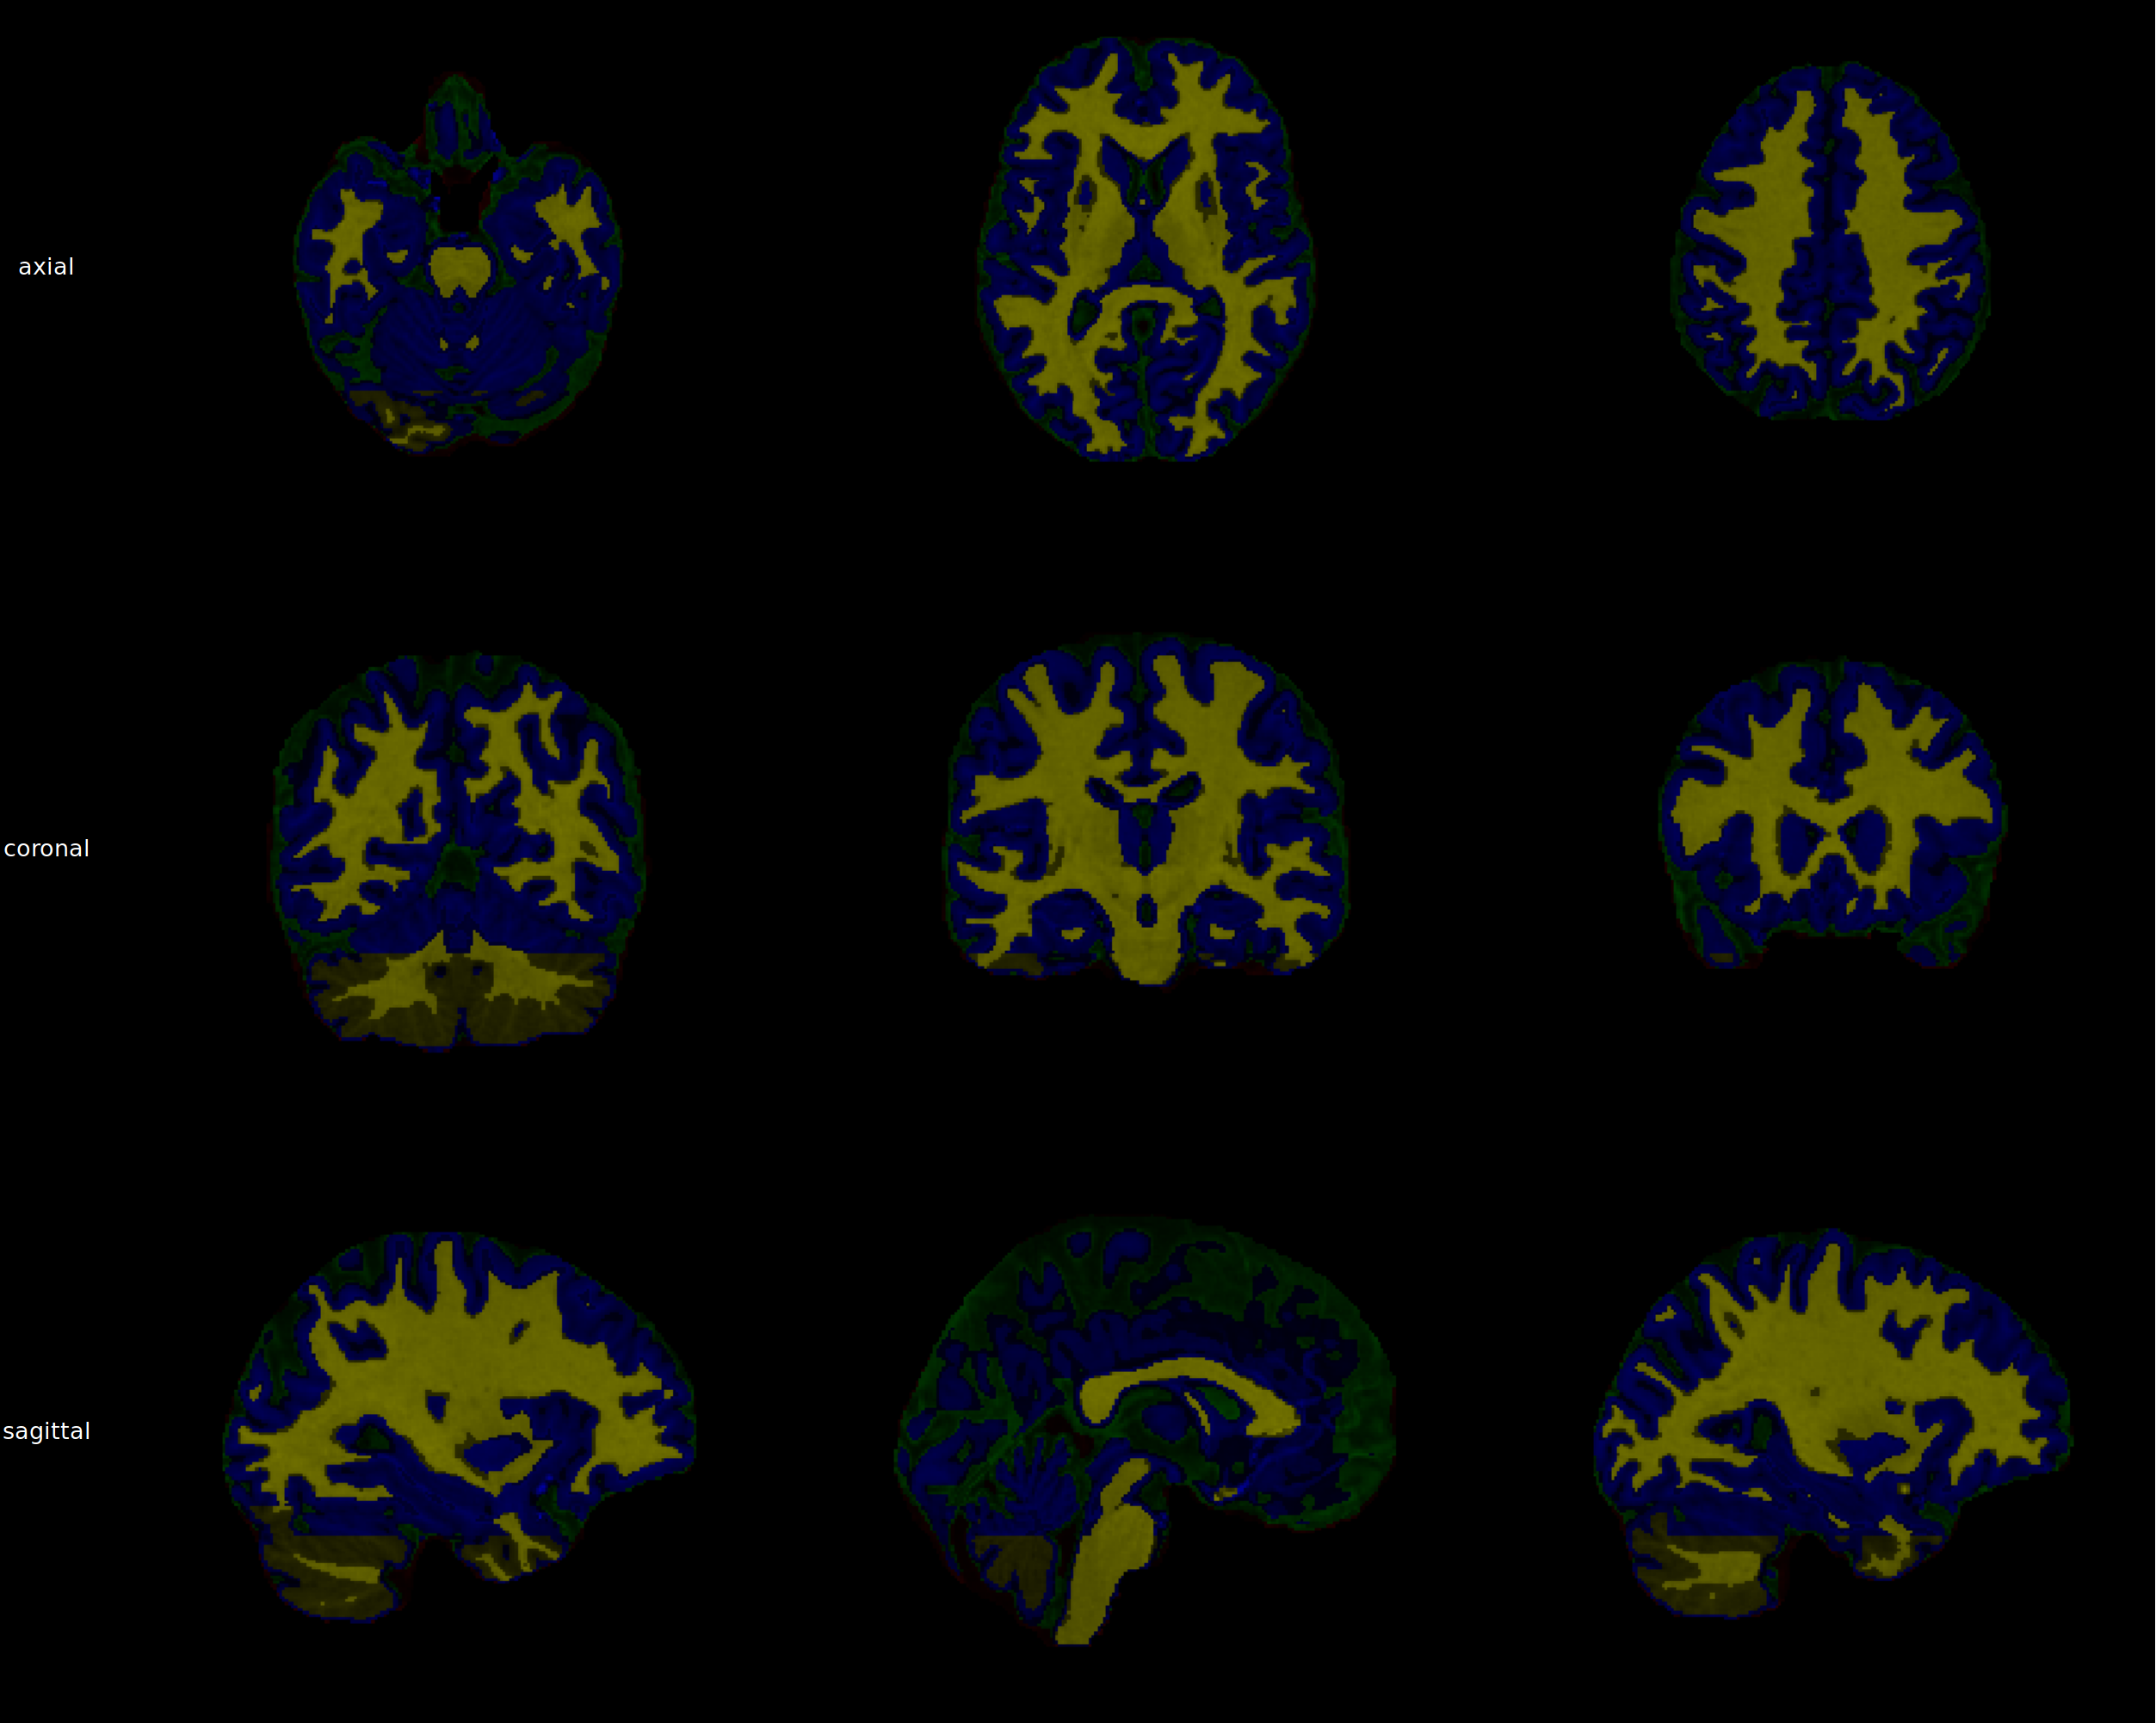
\includegraphics[width=\textwidth]{images/overall_max}
  \caption{Sample slices from the volume with the maximum DICE}
  \label{fig:overall-max-dice}
\end{figure}


\begin{figure}[ht]
  \centering
  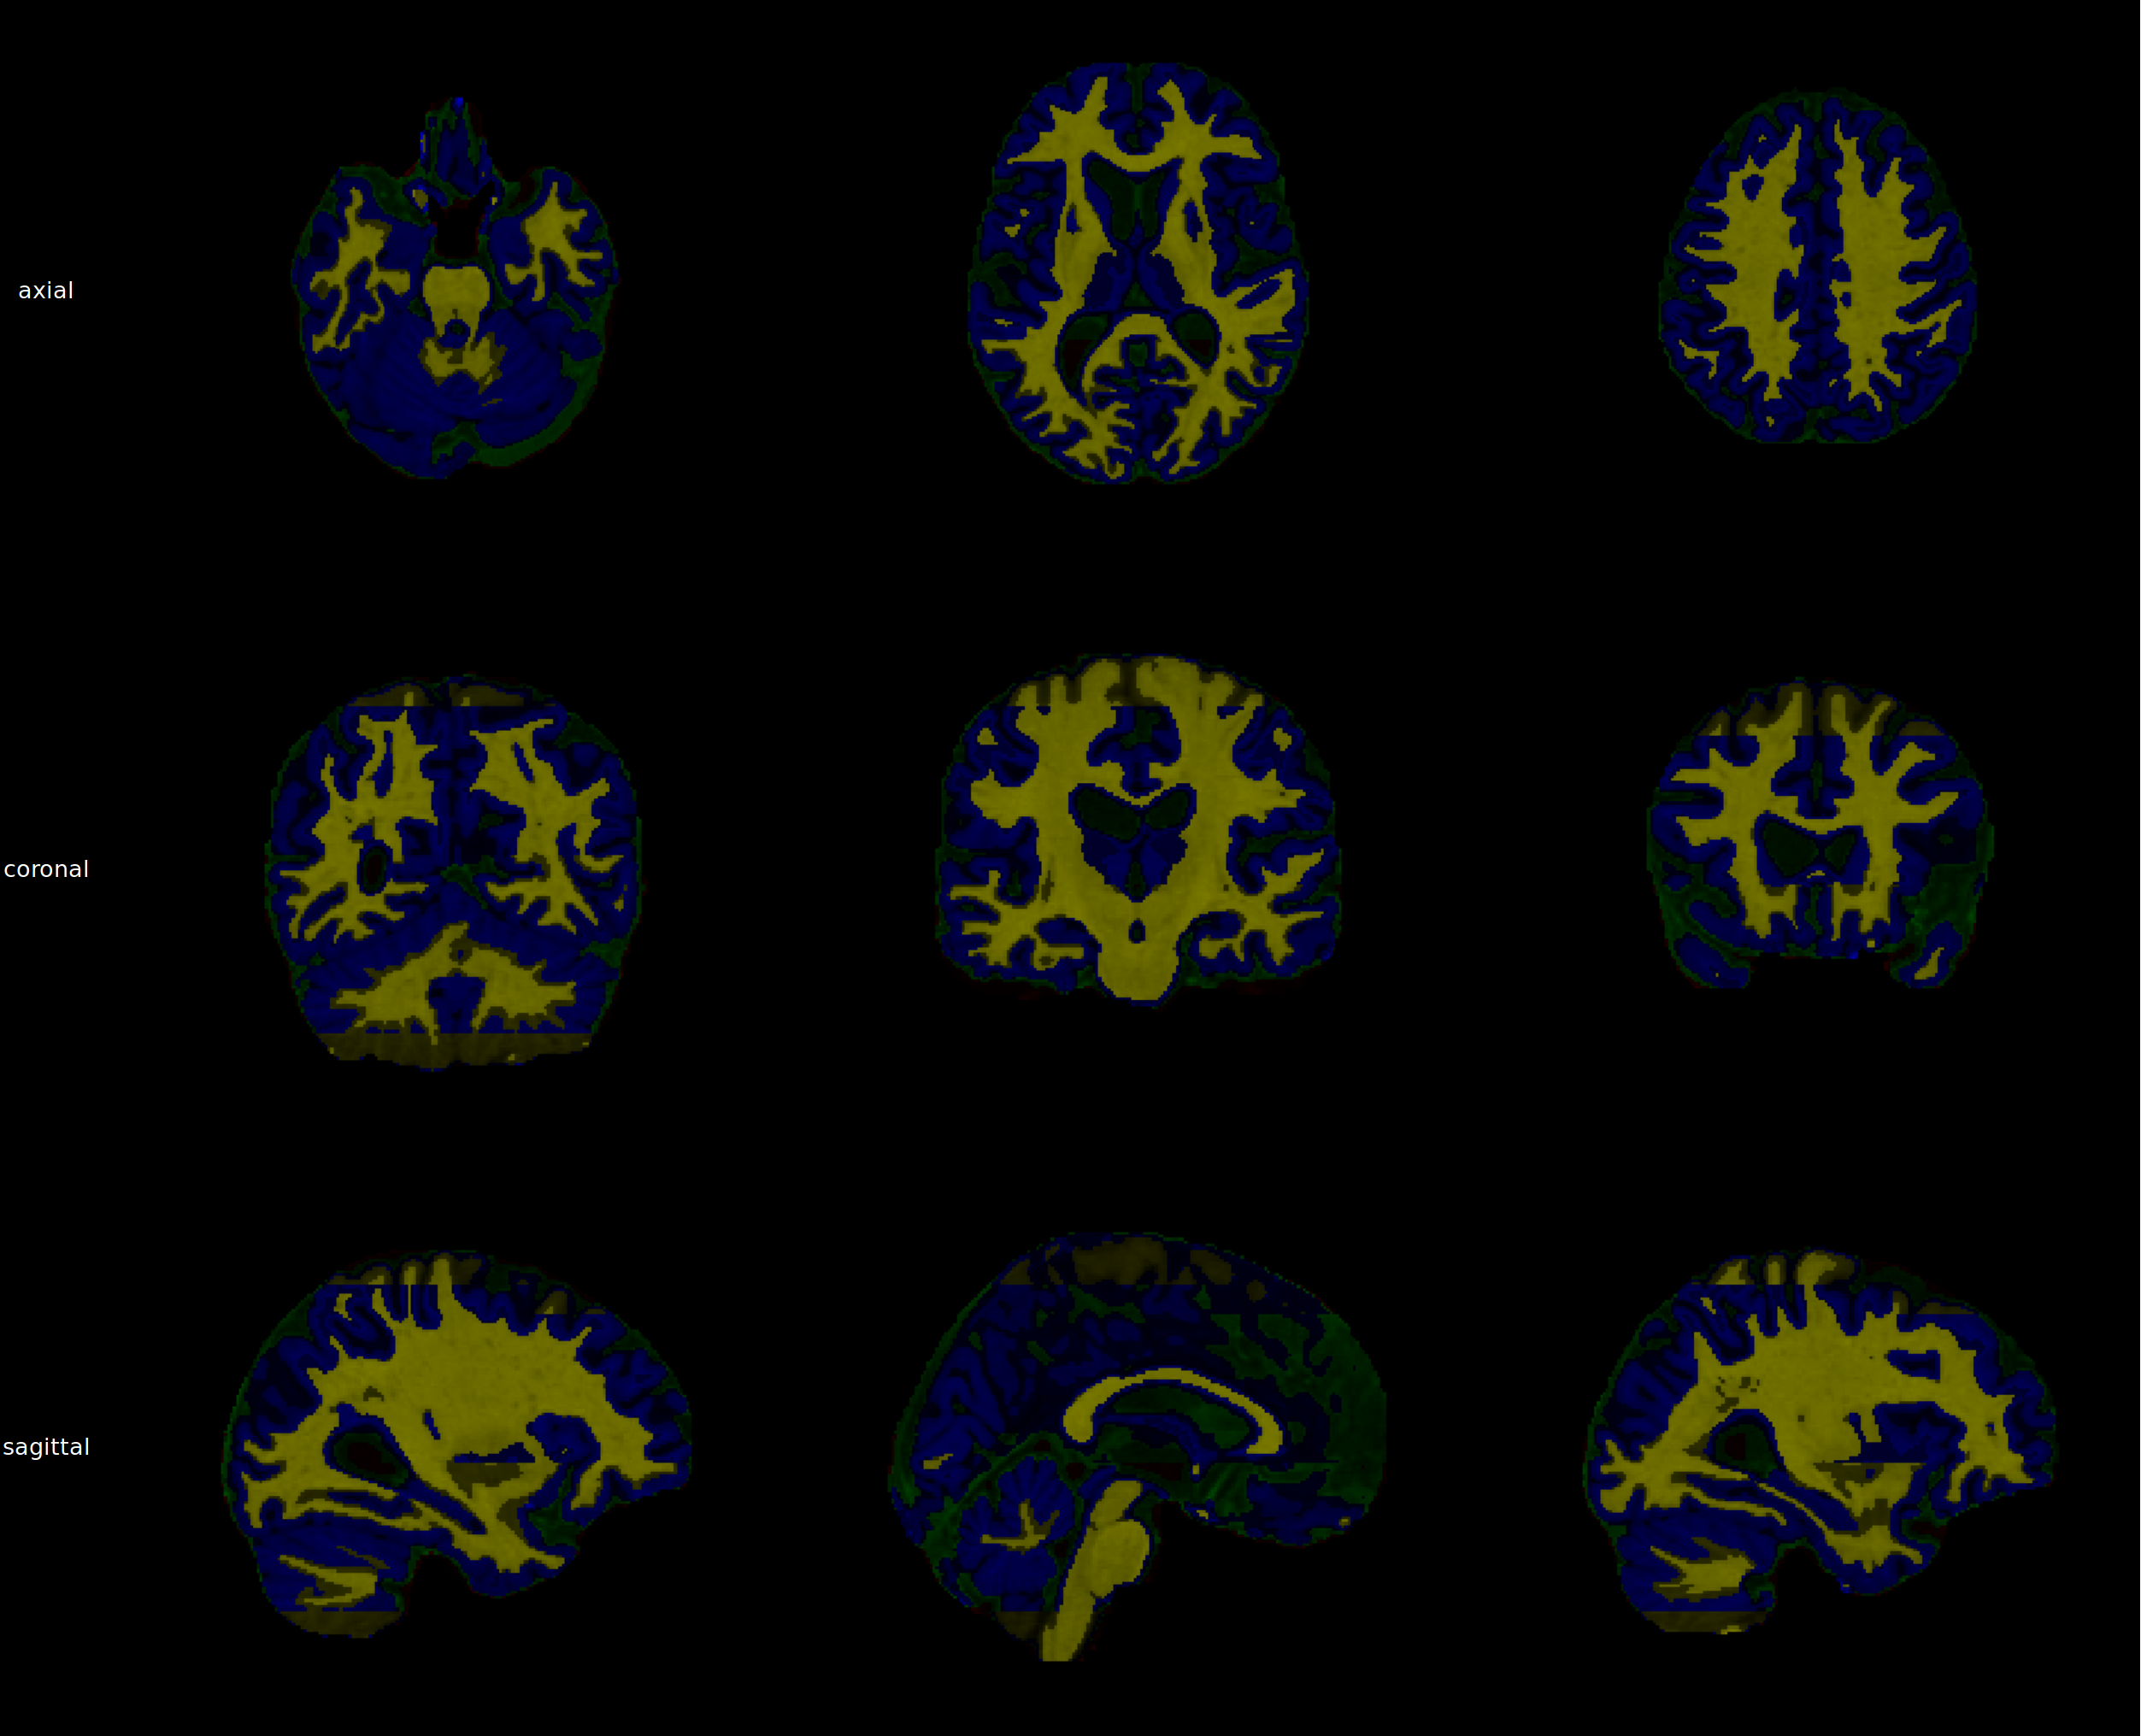
\includegraphics[width=\textwidth]{images/overall_mean}
  \caption{Sample slices from the volume with the mean DICE}
  \label{fig:overall-max-dice}
\end{figure}


\begin{figure}[ht]
  \centering
  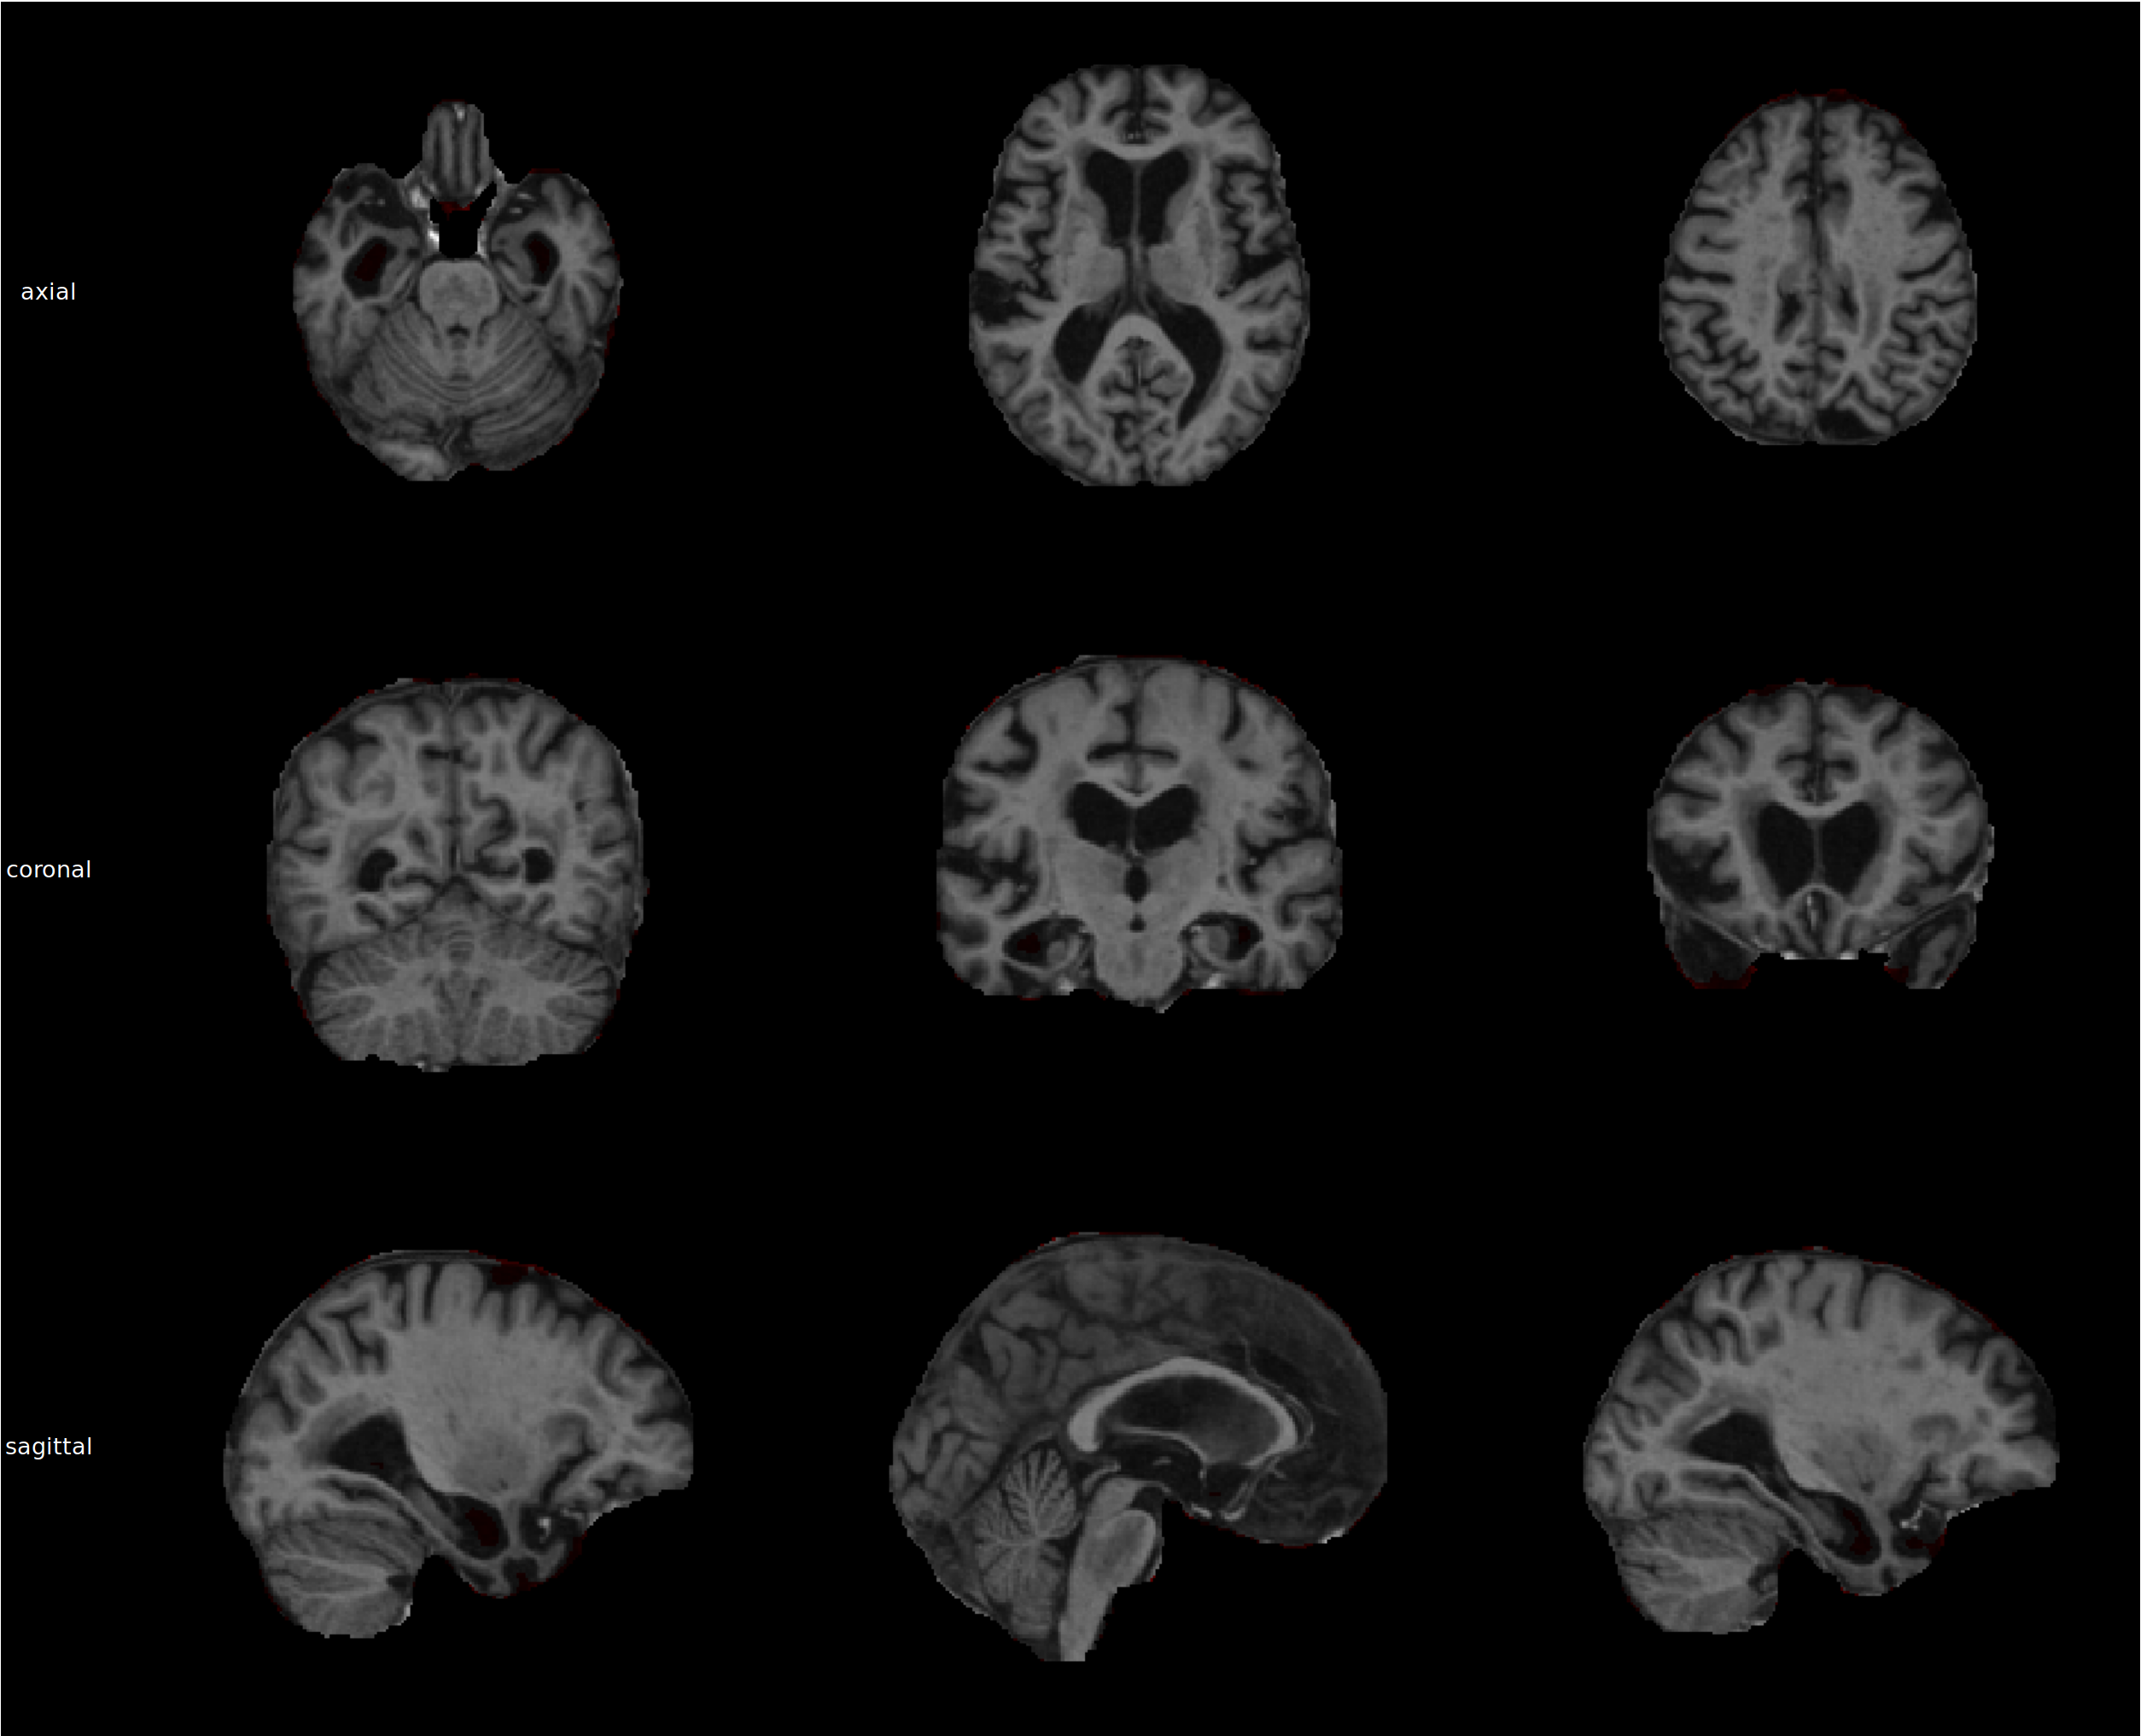
\includegraphics[width=\textwidth]{images/class_0_mean}
  \caption{Sample slices from the volume with the mean DICE for class 0}
  \label{fig:overall-mean-0}
\end{figure}


\begin{figure}[ht]
  \centering
  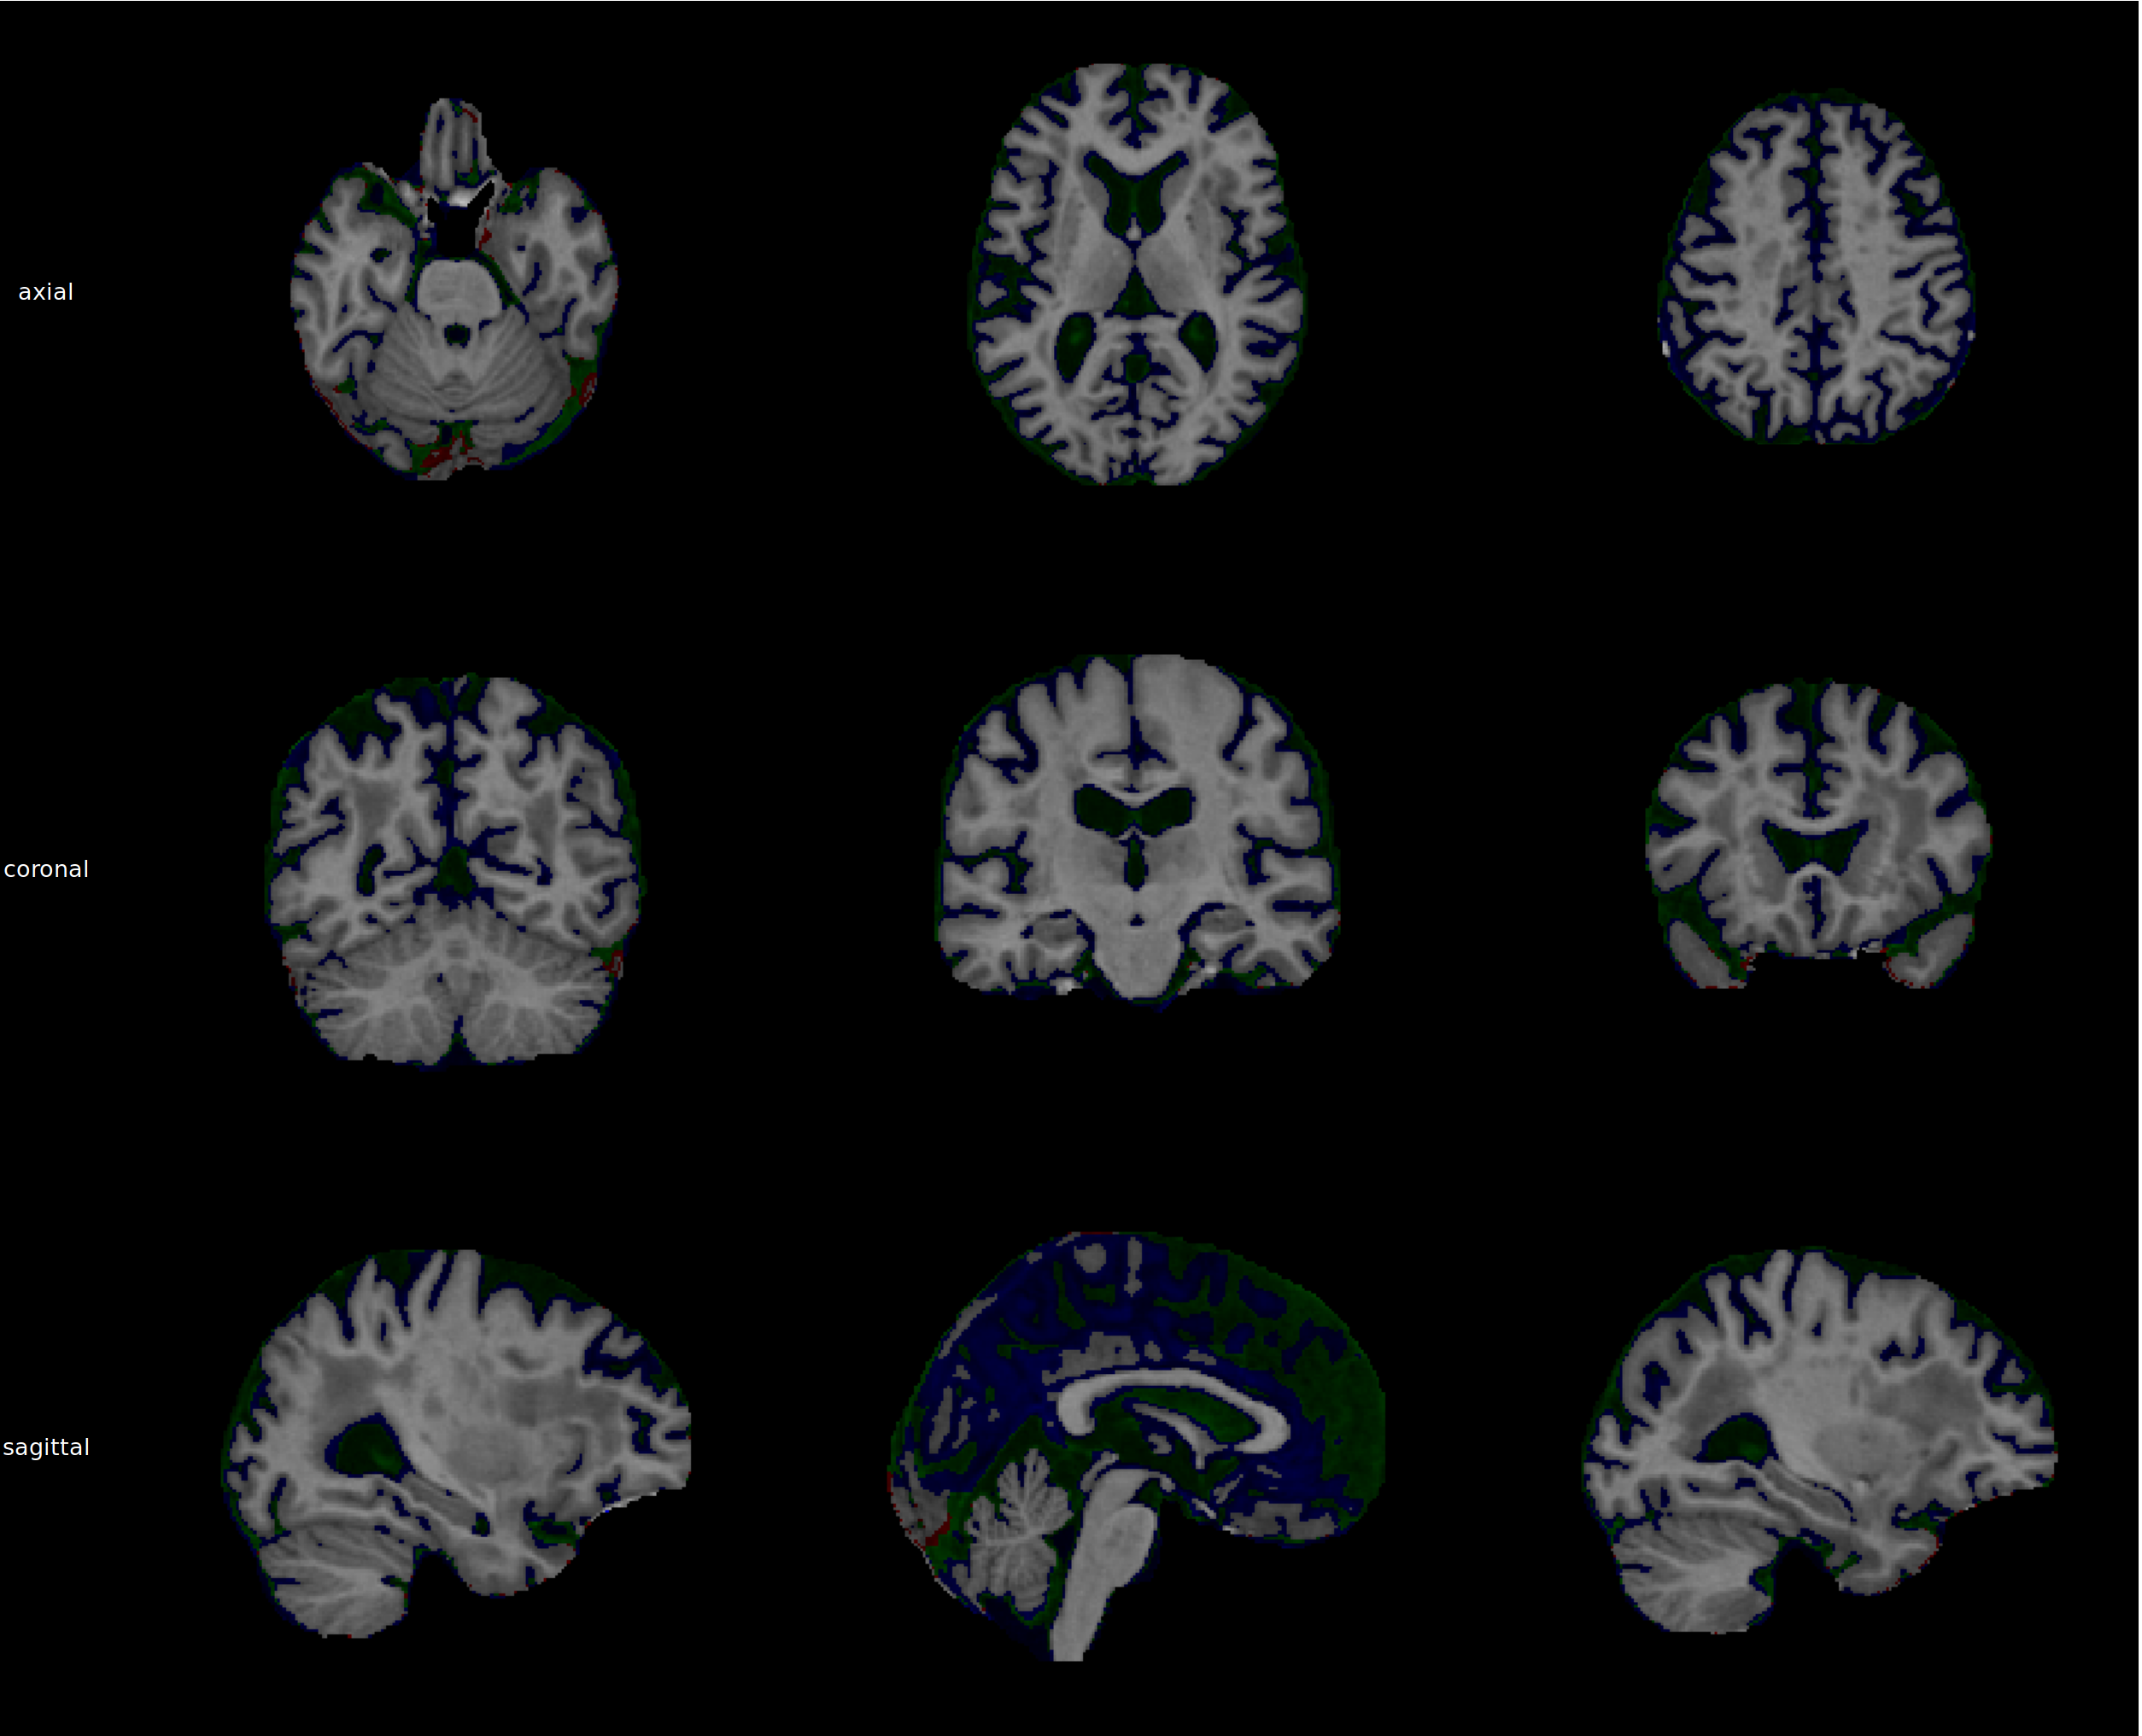
\includegraphics[width=\textwidth]{images/class_1_mean}
  \caption{Sample slices from the volume with the mean DICE for class 1}
  \label{fig:overall-mean-1}
\end{figure}


\begin{figure}[ht]
  \centering
  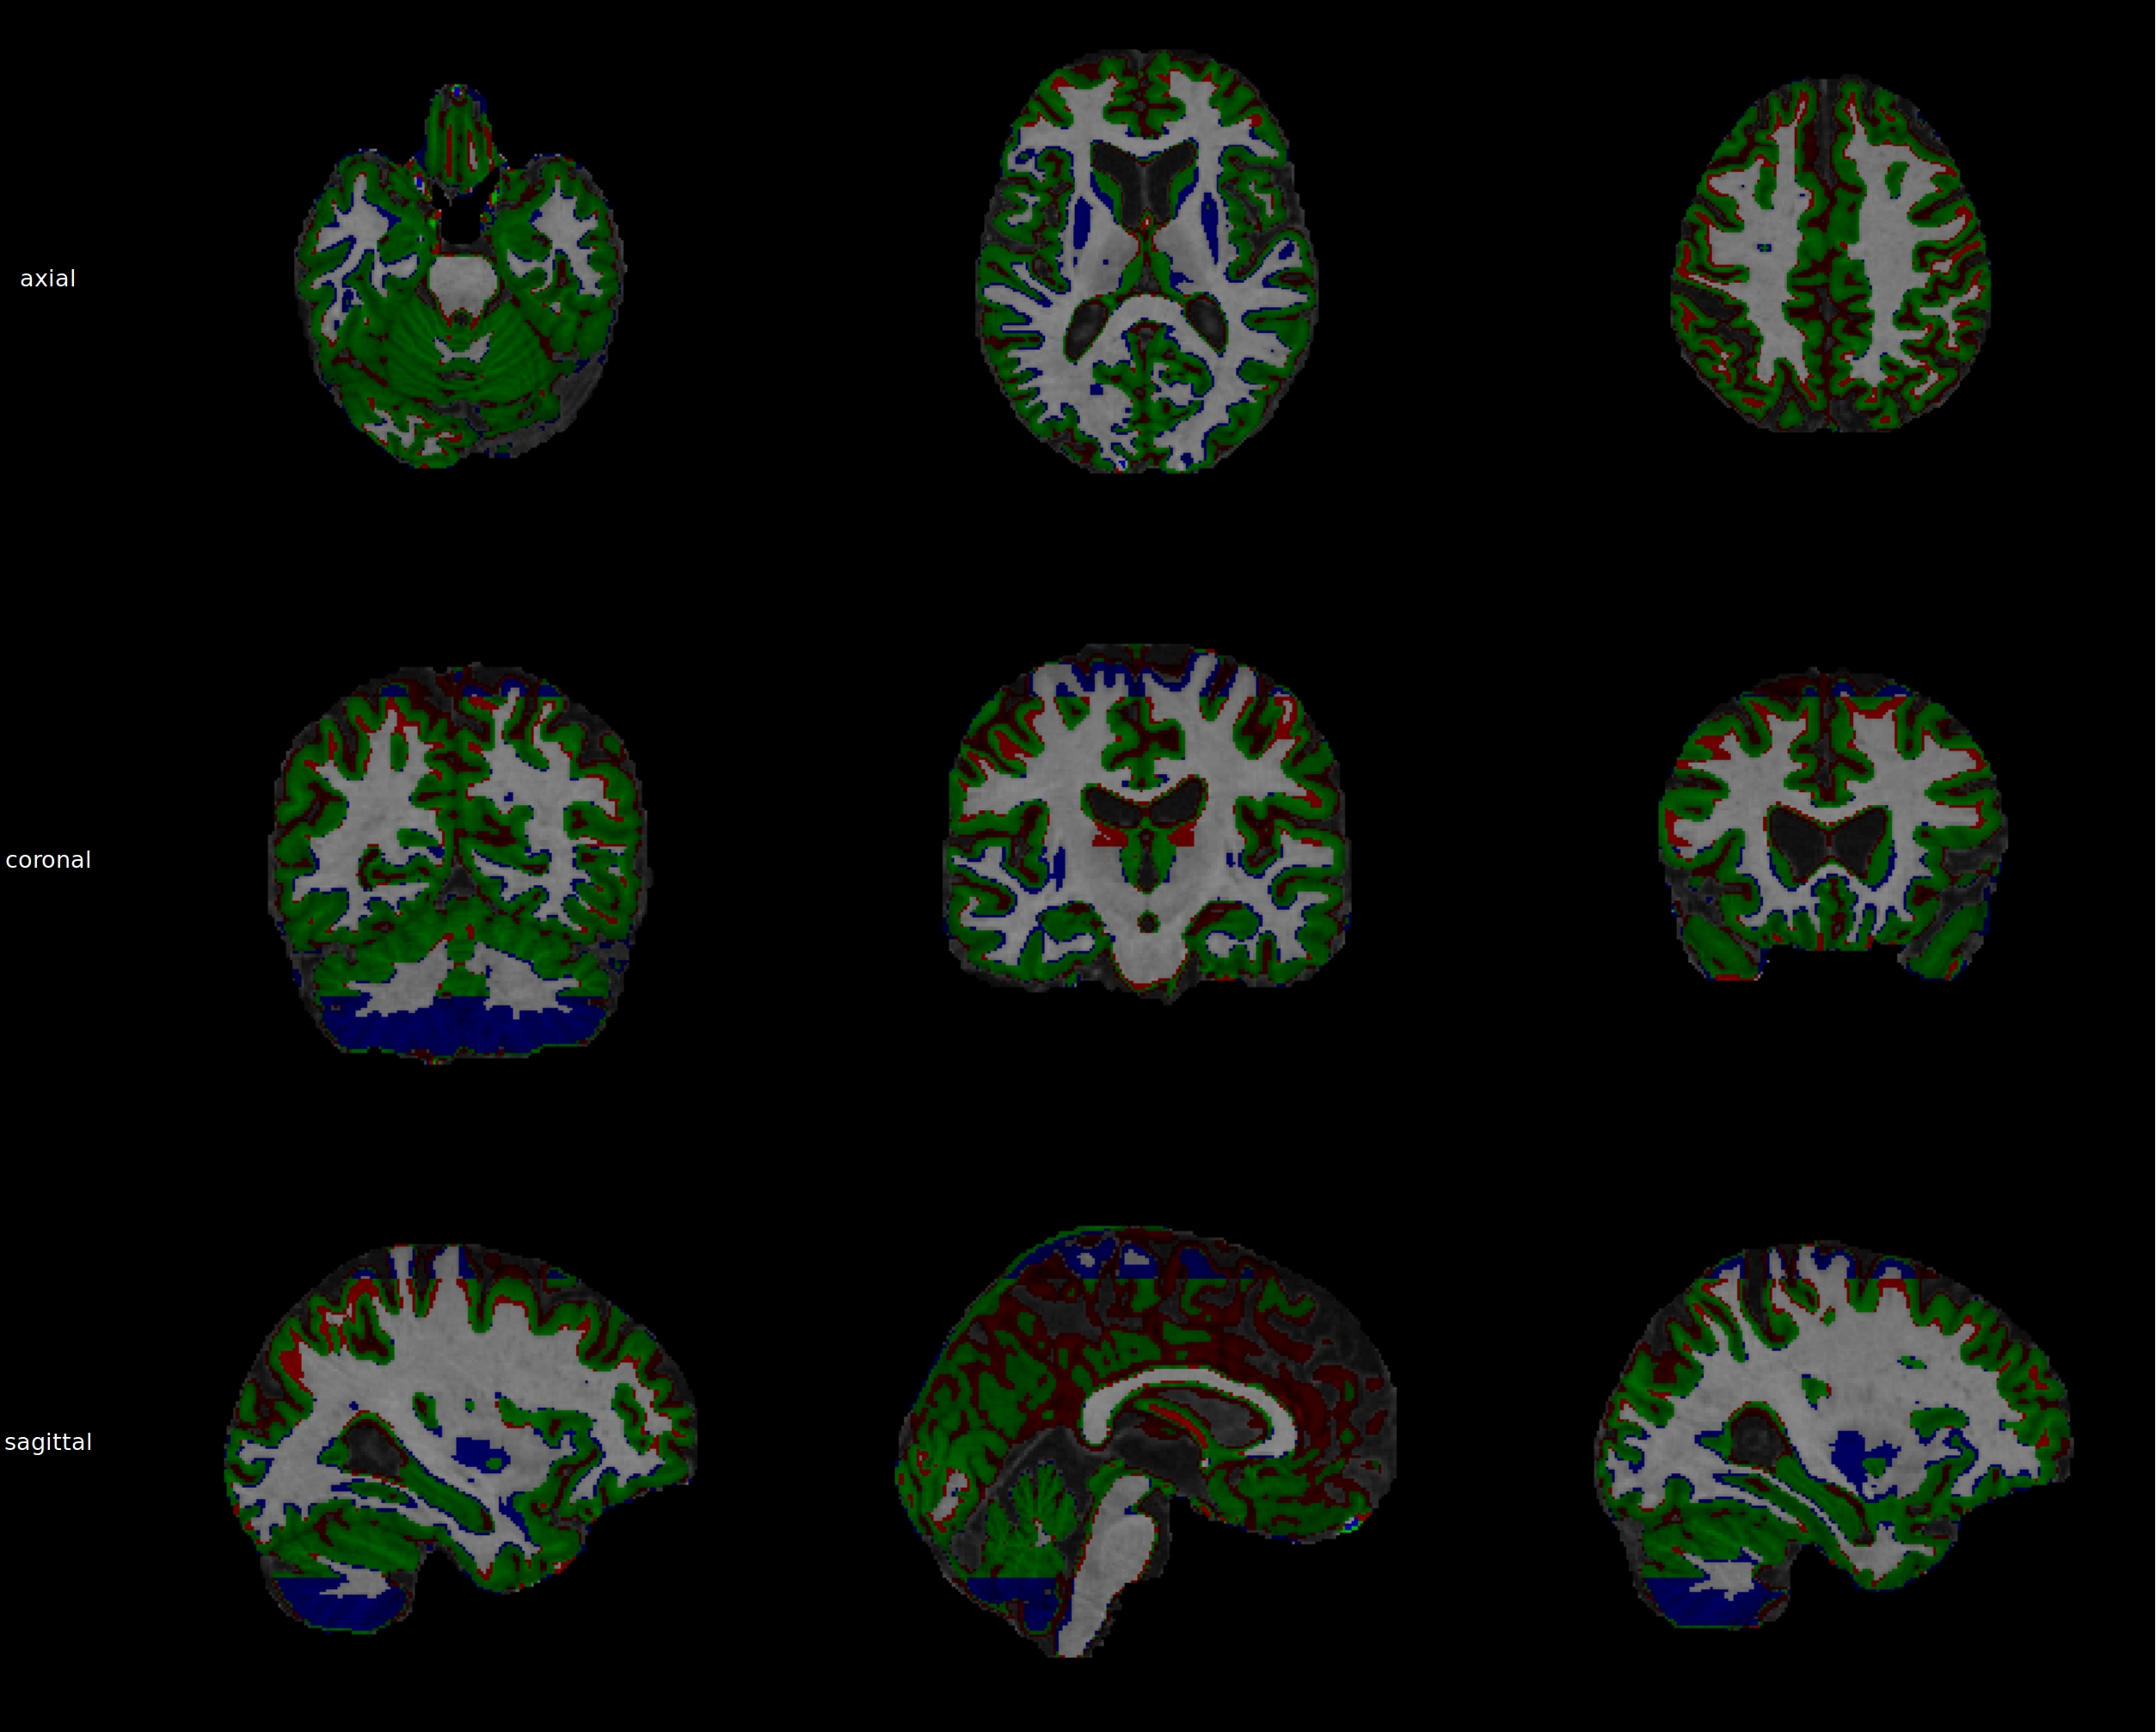
\includegraphics[width=\textwidth]{images/class_2_mean}
  \caption{Sample slices from the volume with the mean DICE for class 2}
  \label{fig:overall-mean-2}
\end{figure}


\begin{figure}[ht]
  \centering
  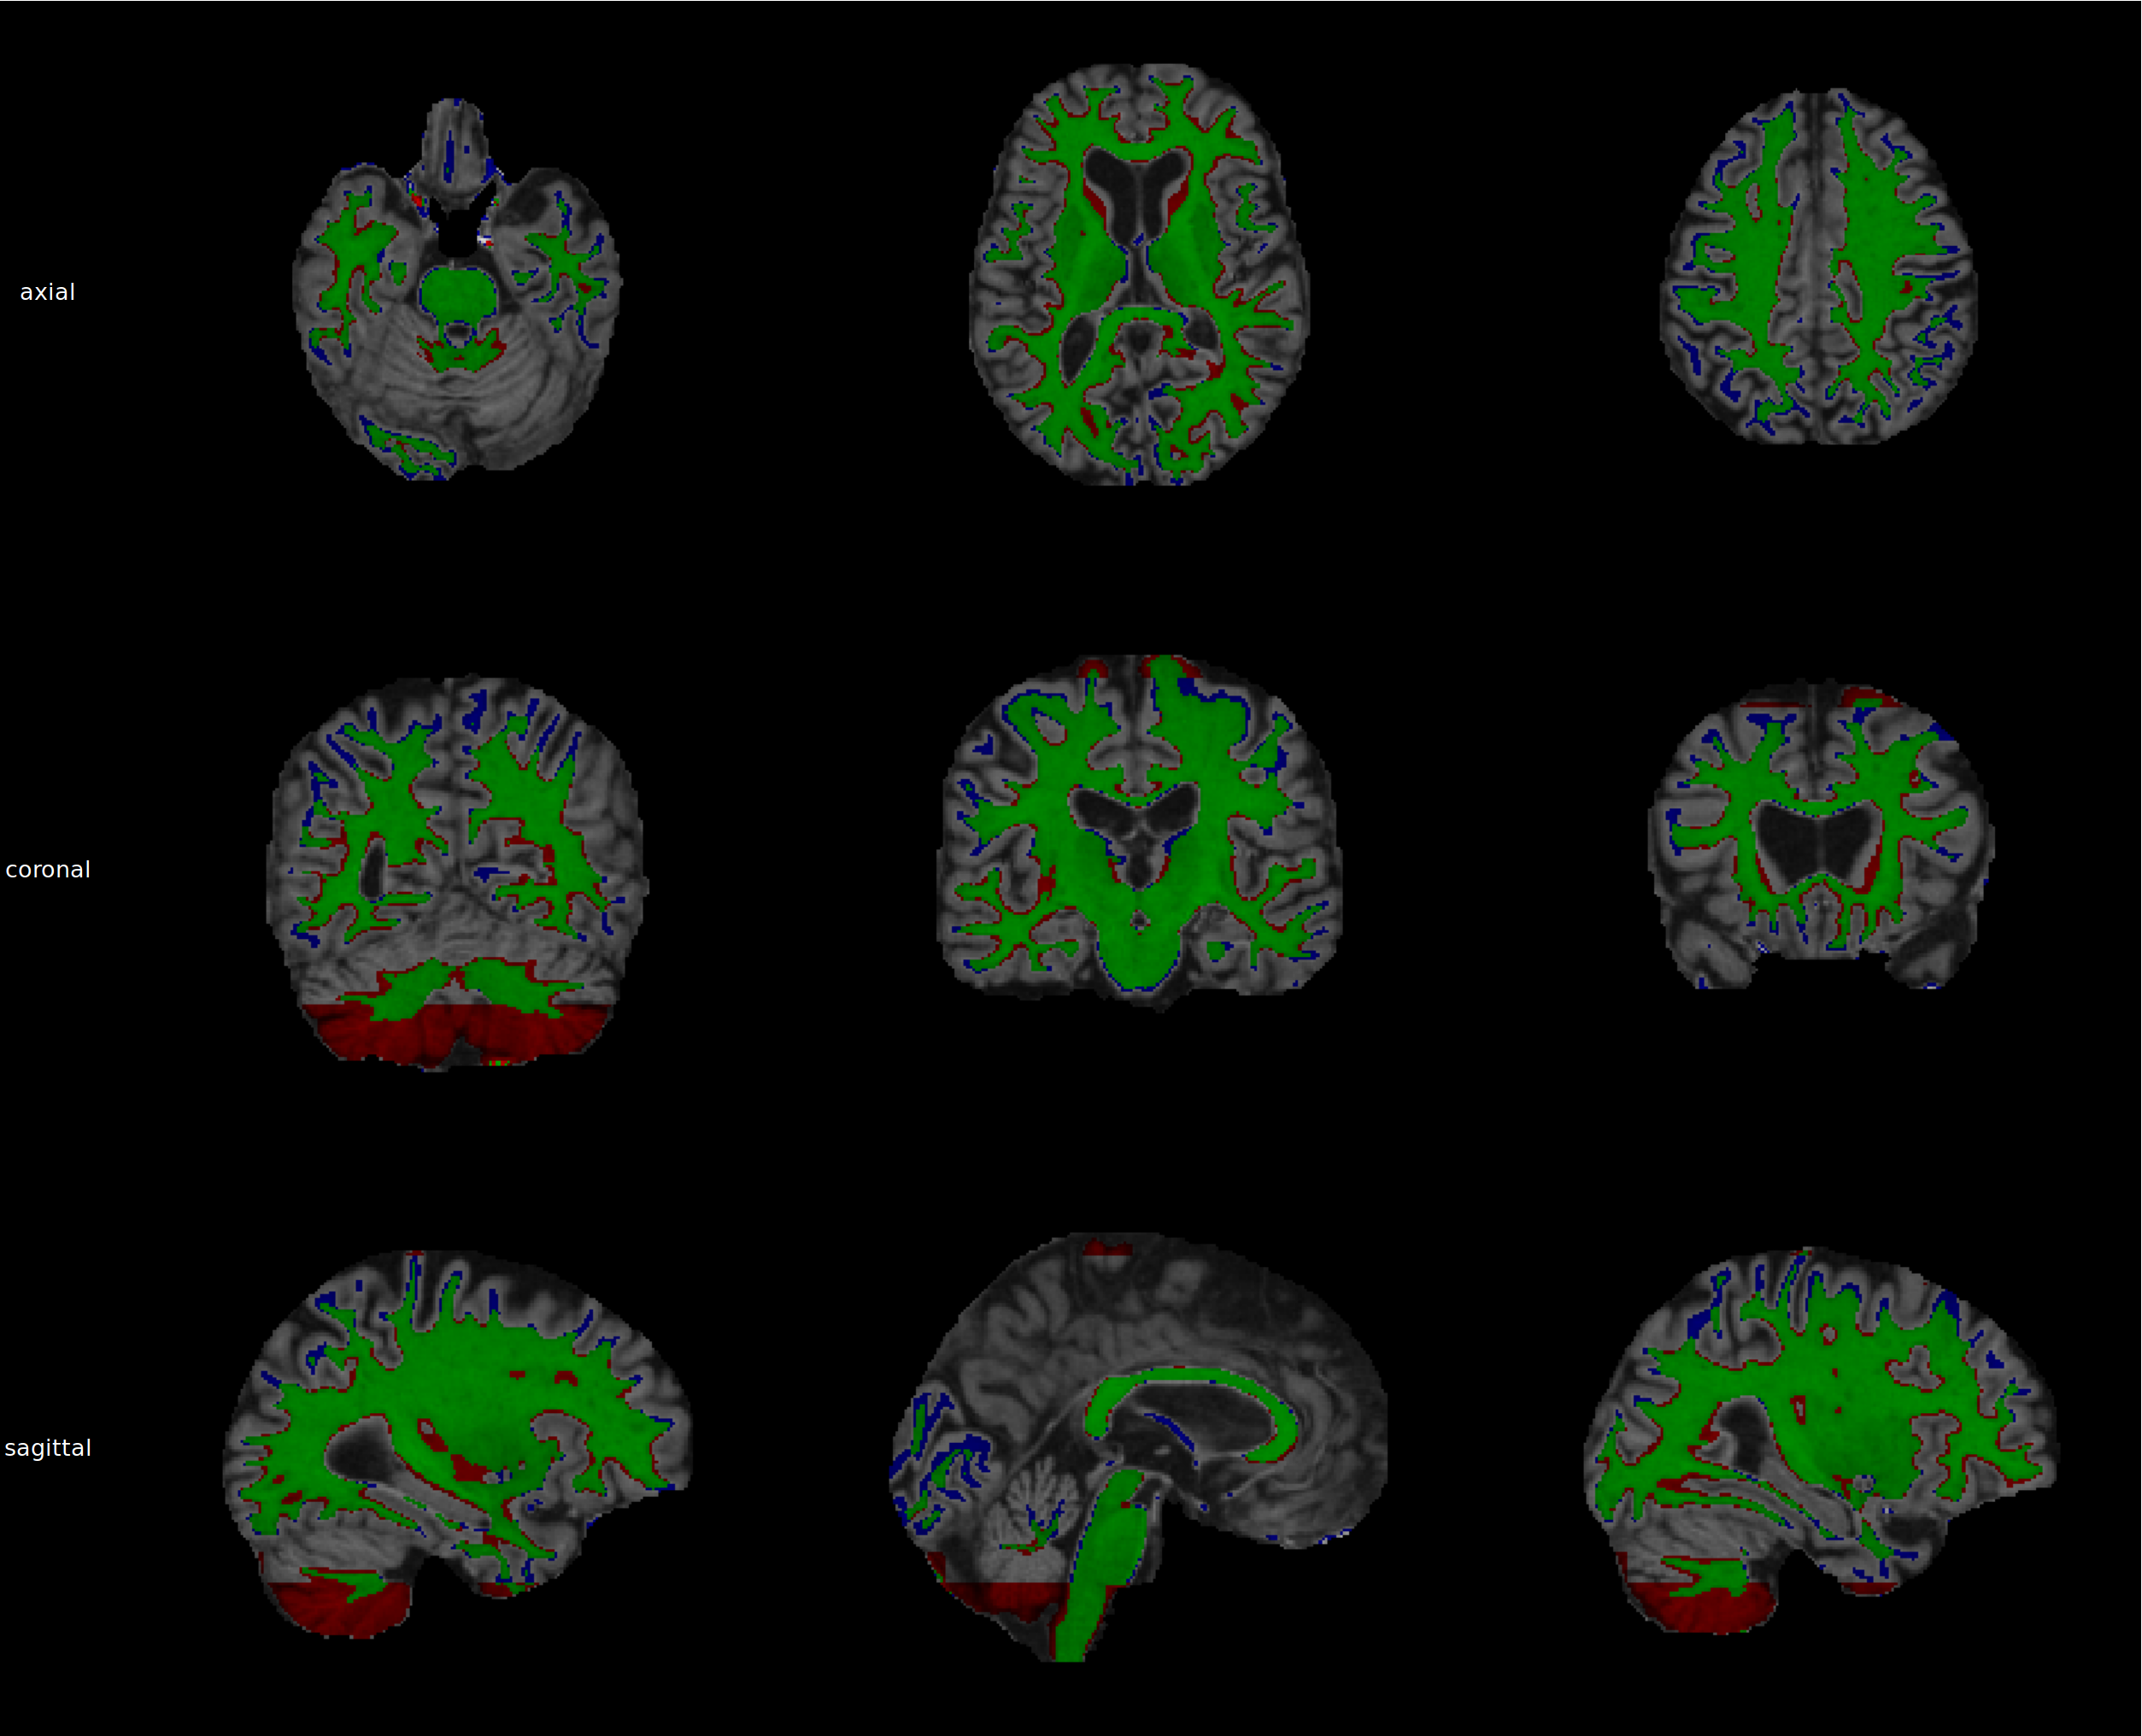
\includegraphics[width=\textwidth]{images/class_3_mean}
  \caption{Sample slices from the volume with the mean DICE for class 3}
  \label{fig:overall-mean-3}
\end{figure}


%===================================================================================================


%%%%%%%%%%%%%%%%%%%%%%%%%%%%%%%%%%%%%%%%%%%%%%%%%%%%%%%%%%%%%%%%%%%%%%%%%%%%%%%%%%%%%%%%%%%%%%%%%%%%
\bibliography{references}
\end{document}
